	\newpage
	\section{PHƯƠNG TRÌNH MẶT CẦU}
	\subsection{LÝ THUYẾT CẦN NHỚ}
	\subsubsection{Khái niệm mặt cầu}
	\begin{enumerate}[\iconMT]
		\item \indam{Định nghĩa:} 
		\begin{boxdn} \immini{Trong không gian, cho trước điểm $I$ và số dương $R$. Mặt cầu tâm $I$ bán kính $R$, kí hiệu $S(I;R)$, là tập hợp tất cả các điểm trong không gian cách điểm $I$ một khoảng bằng $R$. Đoạn thẳng nối hai điểm và đi qua tâm gọi là đường kính của mặt cầu đó.}
			{
		\begin{tikzpicture}[scale=1,>=stealth, font=\footnotesize,line join=round,line cap=round,declare function={a=2; tsai=0.35; b=tsai*a;}]
			\draw[dashed](a,0)coordinate(B) arc (0:180:{a and b});
			\draw (-a,0)coordinate(A) arc (180:360:{a and b});
			\draw (0,0)coordinate(I) circle (a);
			\draw [dashed](A) --(B)($(A)!.5!(I)$)node[above]{$R$};
				\draw [<-,red] ($(I)+(0.05,-0.05)$)--($(I)+(-30:{a+0.4})$)node[below]{tâm};
			\draw [<-,red] ($(I)!0.5!(A)$)--($(I)+(-130:{a+0.6})$)node[below]{bán kính};
			\foreach \t/\g in {I/-90,A/180,B/0}{
				\draw[fill=black] (\t)circle (1pt) node[shift={(\g:7pt)},font=\scriptsize]{$\t$};}
				\end{tikzpicture}
			}
		\end{boxdn}
		\item \indam{Nhận xét:}
		\begin{itemize}
			\item Điểm $M$ thuộc mặt cầu tâm $I$ bán kính $R$ khi và chỉ khi $IM = R$.
			\item Điểm $M$ nằm trong mặt cầu tâm $I$ bán kính $R$ khi và chỉ khi $IM < R$.
			\item Điểm $M$ nằm ngoài mặt cầu tâm $I$ bán kính $R$ khi và chỉ khi $IM > R$.
		\end{itemize}
	\end{enumerate}
	%%%%%%%%%%%%%%%%%%%%%%%%%%%%%%%%%%
	\subsubsection{Phương trình mặt cầu}
		\begin{enumerate}[\iconMT]
		\item \indam{Phương trình mặt cầu:}
		\begin{boxdn}
	 Trong không gian $Oxyz$, mặt cầu $(S)$ tâm $I(a; b; c)$, bán kính $R$ có phương trình là
			$$(x-a)^2 + (y-b)^2 + (z-c)^2 = R^2.$$
		\end{boxdn}
		\item \indam{Nhận xét}
		\begin{itemize}
			\item Phương trình $x^2 + y^2 + z^2 - 2ax - 2by - 2cz + d = 0$ với $a^2 + b^2 + c^2 - d > 0$ là phương trình mặt cầu tâm $I(a; b; c)$, bán kính $R = \sqrt{a^2 + b^2 + c^2 - d}$. 
		\end{itemize}
	\end{enumerate}
	%-------------------------------------------------------------------------------------------------------------
	\subsection{PHÂN LOẠI VÀ PHƯƠNG PHÁP GIẢI TOÁN}
	%Dạng 1
	\begin{dang}{Xác định phương trình mặt cầu}
		%	\begin{listEX}[1]
			%		\item [\ding{172}] Phương trình tổng quát của Parabol 
			%		\item [\ding{172}] 
			%	\end{listEX}
	\end{dang}
	\begin{vd}%[2H5N3-3]%[Dự án đề cương 3 khối NH24-25 Đợt2-Nguyễn Tiến Liên]
		Phương trình nào sau đây là phương trình mặt cầu?
		\choice 
	{$(x-1)^2 + (2y-3)^2 + (z-4)^2 = 192$}
	{$(2x-1)^2 + (y-3)^2 + (z-4)^2 = 192$}
   	{$(x-1)^2 + (y-3)^2 + (3z-4)^2 = 192$}
	{\True $(x-1)^2 + (y-3)^2 + (z-4)^2 = 192$}
\loigiai
{Phương trình $(x-1)^2 + (y-3)^2 + (z-4)^2 = 192$ có dạng phương trình mặt cầu với tâm $I(1;3;4)$, bán kính $R=\sqrt{192}$.}
	\end{vd}
	\begin{vd}%[2H5N3-3]%[Dự án đề cương 3 khối NH24-25 Đợt2-Nguyễn Tiến Liên]
			Phương trình nào sau đây là phương trình mặt cầu?
			\choice 
			{$x^2 + y^2 - z^2- 4x - 3y - 2z - 7=0$}
			{$x^2 + y^2 + z^2+2x + y + 5=0$}
			{$x^2 - y^2 + z^2- 4 x - 3y - 2z - 7=0$}
			{\True $x^2 + y^2 + z^2- 4x - 3y - 2z - 7=0$}
			\loigiai{
				Phương trình $x^2 + y^2 + z^2- 4 x - 3 y - 2 z - 7=0$ là phương trình mặt cầu với $\heva{&\text{tâm } I\left(2;\dfrac{3}{2};1\right)\\& \text{ bán kính } R=\sqrt{2^2+\left(\dfrac{3}{2}\right)^2+1^2-(-7)}=\dfrac{\sqrt{57}}{2}.}$
		}
	\end{vd}
	%%%%%%%%%%%%%%%%%%%%%%%%%%%%%%%%%%%%%%%%%%%%%%%
	%Dạng 2
	\begin{dang}{Xác định tâm, bán kính của mặt cầu}
	\end{dang}
	\begin{vd}%[2H5N3-2]%[Dự án đề cương 3 khối NH24-25 Đợt2-Nguyễn Tiến Liên]
		 Cho mặt cầu có phương trình $(x-8)^2+(y+7)^2+z^2=4$. Tìm tâm và bán kính của mặt cầu đó.
		\loigiai{
			Ta có
			$(x-8)^2+(y+7)^2+z^2=4 \Leftrightarrow (x-8)^2+[y-(-7)]^2+(z-0)^2=2^2$.\\
			Vậy mặt cầu đã cho có tâm $I(8;-7;0)$ và bán kính $R=2.$}
	\end{vd}
	\begin{vd}%[2H5N3-2]%[Dự án đề cương 3 khối NH24-25 Đợt2-Nguyễn Tiến Liên]
	Cho mặt cầu có phương trình $x^2+y^2+z^2-10x+6z+5=0$. Xác định tâm và bán kính của mặt cầu đó.
	\loigiai{
		Ta có $x^2+y^2+z^2-10x+6z+5=0$
		$\Leftrightarrow (x-5)^2+y^2+(z+3)^2=29$.\\
		Vậy mặt cầu đã cho có tâm $I(5;0;-3)$, bán kính $R=\sqrt{29}$. }
	\end{vd}
	\begin{vd}%[2H5N3-2]%[Dự án đề cương 3 khối NH24-25 Đợt2-Nguyễn Tiến Liên]
		Cho hai điểm $A(6;-8;1)$ và $B(0;6;3)$. Xác định tâm $I$ của mặt cầu đường kính $AB$.
	\loigiai{
		Tâm $I(x; y; z)$ là trung điểm của đoạn thẳng $AB$ nên
		$\heva{&x = \dfrac{6+0}{2} = 3\\& y = \dfrac{-8+6}{2} = -1\\& z = \dfrac{1+3}{2} = 2.}$\\
		Vậy $I(3; -1; 2)$.}
	\end{vd}
	%%%%%%%%%%%%%%%%%%%%
	%Dạng 3
	\begin{dang}{Lập phương trình mặt cầu trong các trường hợp đơn giản}
	\end{dang}
	\begin{vd}%[2H5N3-3]%[Dự án đề cương 3 khối NH24-25 Đợt2-Nguyễn Tiến Liên]
	Lập phương trình mặt cầu có tâm $I(0; -12; 3)$ và bán kính $4$.
	\loigiai{
	Phương trình mặt cầu có tâm $I(0; -12; 3)$ và bán kính $4$ là\\
	 $(x-0)^2 + (y-(-12))^2 + (z-3)^2 = 4^2$\\
	$\Leftrightarrow x^2 + (y+12)^2 + (z-3)^2 = 16$.
		} 
	\end{vd}
	\begin{vd}%[2H5H3-3]%[Dự án đề cương 3 khối NH24-25 Đợt2-Nguyễn Tiến Liên]
	Lập phương trình mặt cầu tâm $I(-3; -7; 8)$, biết mặt cầu đi qua điểm $A(-2; -5; 7)$.
	\loigiai{
	Bán kính của mặt cầu đó bằng $IA = \sqrt{(-2-(-3))^2 + (-5-(-7))^2 + (7-8)^2} = \sqrt{6}$.\\
	Vậy phương trình mặt cầu đó là $(x+3)^2 + (y+7)^2 + (z-8)^2 = 6$.
		}
	\end{vd}
	%%%%%%%%%%%%%%%%%%
	%Dạng 4
	\begin{dang}{Lập phương trình mặt cầu đi qua $4$ điểm không đồng phẳng}
		\begin{enumerate}[label=\textbf{B\arabic*.}]
			\item Gọi $I(a; b; c)$ là tọa độ tâm mặt cầu cần tìm.
			\item Mặt cầu $(S)$ đi qua $4$ điểm $A$; $B$; $C$; $D$  $\Leftrightarrow IA = IB = IC = ID \Leftrightarrow \heva{&IA^2 = IB^2 \\& IA^2 = IC^2 \\& IA^2 = ID^2}\\ \Rightarrow$ tọa độ  tâm $I(a; b; c)$ và bán kính $R=IA$ . 
			\item mặt cầu $(S)$ tâm $I(a; b; c)$, bán kính $R$ có phương trình là
			$$(x-a)^2 + (y-b)^2 + (z-c)^2 = R^2.$$
		\end{enumerate}
		\indam{Chú ý:}Có thể giải theo cách khác như sau:
		\begin{itemize}
			\item Gọi phương trình mặt cầu có dạng $(S)\colon x^2 + y^2 + z^2 + 2ax + 2by + 2cz + d = 0$ (với $a^2 + b^2 + c^2 - d > 0$) $\quad (1)$.
			\item Thay tọa độ $4$ điểm $A$; $B$; $C$; $D$ vào phương trình $(1)$ ta được hệ $4$ phương trình $4$ ẩn $a$, $b$, $c$, $d$.
			\item Giải hệ này ta tìm được $a$, $b$, $c$, $d$.
			\item Thay vào phương trình  $(1)$, ta được phương trình mặt cầu cần tìm. 
		\end{itemize}
	\end{dang}
	\begin{vd}%[2H5V3-2]%[Dự án đề cương 3 khối NH24-25 Đợt2-Nguyễn Tiến Liên]
		Trong không gian $Oxyz$, nếu mặt cầu $(S)$ đi qua bốn điểm $M(2;2;2)$, $N(4;0;2)$, $P(4;2;0)$ và $Q(4;2;2)$ thì tâm $I$ của $(S)$ có tọa độ là?
		\loigiai{
			Gọi phương trình mặt cầu có dạng $(S)\colon x^2 + y^2 + z^2 + 2ax + 2by + 2cz + d = 0$ ($a^2 + b^2 + c^2 - d > 0$).\\
			Vì $M$, $N$, $P$, $Q$ $\in (S)$ nên ta có hệ phương trình
			$$ \heva{& 2^2 + 2^2 + 2^2 + 4a + 4b + 4c + d = 0 \\& 4^2 + 0^2 + 2^2 + 8a + 0b + 4c + d = 0 \\& 4^2 + 2^2 + 0^2 + 8a + 4b + 0c + d = 0 \\& 4^2 + 2^2 + 2^2 + 8a + 4b + 4c + d = 0} \Leftrightarrow \heva{& a = -3 \\& b = -1 \\& c = -1 \\& d = 8.} \Rightarrow I(3;1;1) \text{ là tâm mặt cầu }(S).$$
		}
	\end{vd}
	\begin{vd}%[2H5V3-3]%[Dự án đề cương 3 khối NH24-25 Đợt2-Nguyễn Tiến Liên]
		Trong không gian $Oxyz$, cho 4 điểm $A(2;0;0), B(0;2;0), C(0;0;2), D(2;2;2)$. Viết phương trình mặt cầu $(S)$ ngoại tiếp tứ diện $ABCD$.
		\loigiai{
			Gọi phương trình mặt cầu có dạng $x^2 + y^2 + z^2 + 2ax + 2by + 2cz + d = 0$.\\
			Vì mặt cầu ngoại tiếp tứ diện $ABCD$ nên tọa độ các điểm $A$, $B$, $C$, $D \in (S)$.
			Ta có:
			$$ \heva{&4 + 4a + d = 0 \\& 4 + 4b + d = 0 \\& 4 + 4c + d = 0 \\& 12 + 4a + 4b + 4c + d = 0} \Leftrightarrow \heva{& a = -1 \\& b = -1 \\& c = -1 \\& d = 0.} $$
			Suy ra phương trình mặt cầu là $x^2 + y^2 + z^2 - 2x - 2y - 2z = 0$.
		}
	\end{vd}
		%%%%%%%%%%%%%%%%%%
	%Dạng 5
	\begin{dang}{Lập phương trình mặt cầu, biết mặt cầu $(S)$ có tâm $I(a;b;c)$ và tiếp xúc với mặt phẳng $(P)\colon Ax + By + Cz + D = 0$ }
		\begin{enumerate}[label=\textbf{B\arabic*.}]
			\item Gọi $R$ là bán kính mặt cầu cần tìm.\\
		 Mặt cầu $(S)$ tiếp xúc với mặt phẳng $(P)$ nên $R=\mathrm{d}(I,(P)) = \dfrac{\left|Aa+Bb+Cc+D\right|}{\sqrt{A^2+B^2+C^2}}$. 
			\item Mặt cầu $(S)$ tâm $I(a; b; c)$, bán kính $R$ có phương trình là
			$$(x-a)^2 + (y-b)^2 + (z-c)^2 = R^2.$$
		\end{enumerate}
		\indam{Chú ý:}
			\begin{itemize}
			\item Nếu $(S)$ tâm $I(a;b;c)$ tiếp xúc với $(Oxy)$ thì $R=|c|$.
			\item Nếu $(S)$ tâm $I(a;b;c)$ tiếp xúc với $(Oyz)$ thì $R=|a|$.
			\item Nếu $(S)$ tâm $I(a;b;c)$ tiếp xúc với $(Ozx)$ thì $R=|b|$.
		\end{itemize}
	\end{dang}
	\begin{vd}%[2H5H3-3]%[Dự án đề cương 3 khối NH24-25 Đợt2-Nguyễn Tiến Liên]
 Trong không gian $Oxyz$, mặt cầu có tâm $I(1;2;-1)$ và tiếp xúc với mặt phẳng $(P)\colon 2x-2y-z-8=0$ có phương trình $(S)\colon x^2+y^2+z^2-2ax-2by-2cz+d=0$. Tính giá trị của biểu thức $a+b+c+2d$.
\loigiai{
	Bán kính mặt cầu là
	$R = \mathrm{d}(I,(P)) = \dfrac{|2-4+1-8|}{\sqrt{4+4+1}} = 3$.\\
	Phương trình mặt cầu $(S)\colon (x-1)^2+(y-2)^2+(z+1)^2=9$.\\
	$\Leftrightarrow x^2+y^2+z^2-2x-4y+2z-3=0$.\\
	Suy ra $a=1$; $b=2$; $c=-1$; $d=-3$.\\
	Hay $a+b+c+2d = 1+2+(-1)+2\cdot(-3) = -4$.
	}
	\end{vd}
	\begin{vd}%[2H5H3-3]%[Dự án đề cương 3 khối NH24-25 Đợt2-Nguyễn Tiến Liên]
		Trong không gian $Oxyz$, lập phương trình mặt cầu tâm $I(4;-3;-4)$ và tiếp xúc với mặt phẳng $(Oyz)$.\loigiai{ 
			Do mặt cầu tiếp xúc với mặt phẳng $(Oyz) \Rightarrow$ bán kính $R=\mathrm{d}(I,(Oyz))=\sqrt{{x_I}^2}=\sqrt{4^2}=4$.\\ 
			Vậy phương trình mặt cầu cần tìm $\left(x - 4\right)^{2}+\left(y + 3\right)^{2}+\left(z + 4\right)^{2}=16$.}
	\end{vd}
	%%%%%%%%%%%%%%%%%%%%%%%%%%%%%%%%%%%%%%
		%Dạng 6
	\begin{dang}{Mặt cầu cắt mặt phẳng}
		\begin{enumerate}[label=\textbf{B\arabic*.}]
			\item Gọi $(S)$ là mặt cầu  tâm $I(a;b;c)$, bán kính $R$ và $(P)\colon Ax + By + Cz + D = 0$ (hoặc $(P)$ là một trong các mặt phẳng $(Oxy), (Oxz), (Oyz)$).\\
		  Nếu $(S)$ cắt mặt phẳng $(P)$ theo giao tuyến là đường tròn tâm $H$ bán kính $r$\\
		  thì $R^2 = \mathrm{d}^2(I;(P)) + r^2$ $\quad (1)$, với $\mathrm{d}(I;(P)) = \dfrac{\left|Aa + Bb + Cc + D\right|}{\sqrt{A^2 + B^2 + C^2}}$ là khoảng cách từ $I$ đến $(P)$.    
		  \item Sử dụng $(1)$ ta sẽ giải quyết được bài toán.
		\end{enumerate}
		\indam{Chú ý:}
		Trong trường hợp $I$ tiếp xúc một trong các mặt phẳng $(Oxy)$, $(Oxz)$, $(Oyz)$ bài toán sẽ đơn giản hơn.
		
	\end{dang}
		\begin{vd}%[2H5H3-2]%[Dự án đề cương 3 khối NH24-25 Đợt2-Nguyễn Tiến Liên]
		Trong không gian $Oxyz$, cho mặt cầu $(S)\colon (x-2)^2 + (y+3)^2 + (z-4)^2 = 25$. Mặt phẳng $(Oxy)$ cắt mặt cầu $(S)$ có giao tuyến là một đường tròn có bán kính bằng bao nhiêu?
		\loigiai{ 
		Mặt cầu $(S)$ có tâm $I(2;-3;4)$, $R=5$.\\
		Gọi $H$ là tâm đường tròn cắt mặt cầu $(S)$ nên $H$ là hình chiếu của $I$.\\
		 Vậy $H(2;-3;0)$.
		Bán kính đường tròn: $r = \sqrt{R^2 - IH^2} = \sqrt{5^2 - 4^2} = 3$.
		}
	\end{vd}
	\begin{vd}%[2H5H3-3]%[Dự án đề cương 3 khối NH24-25 Đợt2-Nguyễn Tiến Liên]
		Trong không gian $Oxyz$, cho điểm $I(2;4;1)$ và mặt phẳng $(P)\colon x+y+z-4=0$. Tìm phương trình mặt cầu $(S)$ tâm $I$ sao cho $(S)$ cắt $(P)$ theo đường tròn có đường kính bằng $2$.
		\loigiai{
			Ta có $\mathrm{d}(I,(P))=\dfrac{|2+4+1-4|}{\sqrt{1^2+1^2+1^2}}=\sqrt{3}$.\\
			Gọi $R$ là bán kính mặt cầu, ta có $R^2=\mathrm{d}^2(I,(P))+r^2=3+1=4$.\\
			$\Rightarrow (S)\colon (x-2)^2+(y-4)^2+(z-1)^2=4$.}
	\end{vd}
		%Dạng 7
	\begin{dang}{Ứng dụng thực tế}
		\begin{itemize}
			\item Xác định phần hình phẳng quay quanh trục $Ox$.
			\item Sử dụng công thức tính thể tích khối tròn xoay. 
		\end{itemize}
	\end{dang}
	\begin{vd}%[2H5V3-4]%[Dự án đề cương 3 khối NH24-25 Đợt2-Nguyễn Tiến Liên]
		Hệ thống định vị toàn cầu (tên tiếng Anh là Global Positioning System, viết tắt là GPS) là một hệ thống cho phép xác định chính xác vị trí của một vật thể trong không gian (Hình bên dưới). Ta có thể mô phỏng cơ chế hoạt động của hệ thống GPS trong không gian như sau: Trong cùng một thời điểm, tọa độ của một điểm $M$ trong không gian sẽ được xác định bởi bốn vệ tinh cho trước, trên mỗi vệ tinh có một máy thu tín hiệu. Bằng cách so sánh sự sai lệch về thời gian từ lúc tín hiệu được phát đi với thời gian nhận hồi tín hiệu đó, mỗi máy thu tín hiệu xác định được khoảng cách từ vệ tinh đến vị trí $M$ cần tìm tọa độ. Như vậy, điểm $M$ là giao điểm của bốn mặt cầu với tâm lần lượt là bốn vệ tinh đã cho. Giả sử trong không gian với hệ tọa độ $Oxyz$, cho bốn vệ tinh $A(3; -1; 6)$, $B(1; 4; 8)$, $C(7; 9; 6)$, $D(7; -15; 18)$. Tìm tọa độ của điểm $M$ trong không gian, biết khoảng cách từ các vệ tinh đến điểm $M$ lần lượt là $MA = 6$, $MB = 7$, $MC = 12$, $MD = 24$.
		\begin{center}
			
\begin{tikzpicture}[scale=0.5,>=stealth, font=\footnotesize,line join=round,line cap=round]
				%%%%Trái đất
					\tikzset{traidat/.pic={
					\shade[ball color=blue!80!black] (1.12,1.34) circle (2);
				\shade[ball color=green!90!black] (1.6,3.16) .. controls +(-18:0.68) and +(98:0.72) ..
				(2.84,1.66) -- (2.78,1.68) .. controls +(-120:0.1) and +(90:0.1) ..
				(2.82,1.38) .. controls +(-90:0.02) and +(90:0.02) ..
				(2.74,1.28) -- (2.66,1.4) -- (2.66,1.24) -- (2.62,1.24) -- (2.6,1.52) -- (2.54,1.52) -- (2.48,1.72) -- (2.26,1.48) -- (2.26,1.32) -- (2.2,1.28) -- (2.12,1.7) -- (2.08,1.66) -- (1.96,1.8) -- (1.82,1.8) -- (1.76,1.88) -- (1.7,1.84) -- (1.58,1.98) -- (1.56,1.96) -- (1.64,1.78) -- (1.72,1.78) -- (1.72,1.82) -- (1.76,1.82) .. controls +(-50:0.4) and +(14:0.14) ..
				(1.46,1.4) .. controls +(-90:0.2) and +(180:0.08) ..
				(1.64,1.36) .. controls +(-90:0.18) and +(54:0.16) ..
				(1.34,0.82) -- (1.38,0.56) .. controls +(-79:0.06) and +(63:0.08) ..
				(1.22,0.36) -- (1.22,0.26) -- (1.16,0.22) .. controls +(-96:0.1) and +(0:0.1) ..
				(0.94,0) -- (0.8,0) .. controls +(90:0.16) and +(-120:0.3) ..
				(0.74,0.68) .. controls +(60:0.1) and +(-90:0.02) ..
				(0.64,0.96) -- (0.64,1.12) -- (0.56,1.12) .. controls +(104:0.04) and +(0:0.04) ..
				(0.5,1.18) -- (0.46,1.18) .. controls +(190:0.4) and +(-90:0.1) ..
				(0,1.42) -- (0,1.68) .. controls +(90:0.1) and +(-146:0.08) ..
				(0.16,1.96) -- (0.16,2.06) -- (0.26,2.16) -- (0.32,2.16) .. controls +(0:0.12) and +(180:0.08) ..
				(0.5,2.24) -- (0.68,2.24) -- (0.68,2.08) -- (0.88,2) -- (0.92,2.08) .. controls +(-16:0.08) and +(180:0.1) ..
				(1.14,2.02) -- (1.18,2.02) .. controls +(0:0.08) and +(-90:0.08) ..
				(1.28,2.2) -- (1.1,2.18) -- (1.04,2.36) -- (0.94,2.32) .. controls +(-68:0.06) and +(0:0.04) .. (0.94,2.2) -- (0.86,2.38) -- (0.7,2.5) -- (0.68,2.48) -- (0.82,2.34) .. controls +(-117:0.06) and +(-53:0.12) ..
				(0.72,2.24) -- (0.8,2.28) -- (0.62,2.46) -- (0.52,2.42) -- (0.4,2.32) .. controls +(-98:0.08) and +(-10:0.2) .. (0.2,2.24) -- (0.2,2.44) -- (0.38,2.44) -- (0.32,2.58) -- (0.3,2.56) -- (0.3,2.6) -- (0.6,2.74) .. controls +(90:0.04) and +(-90:0.04) ..
				(0.58,2.82) .. controls +(0:0) and +(0:0) ..
				(0.62,2.86) -- (0.7,2.8) -- (0.68,2.9) -- (0.56,2.88) -- (0.52,2.98) .. controls +(27:0.1) and +(180:0.08) ..
				(0.92,3.22) -- (0.98,3.22) .. controls +(0:0.08) and +(124:0.04) ..
				(1.24,3.12) -- (1.08,3.14) -- (1.2,3.04) -- (1.22,3.08) -- (1.3,3.1) -- (1.3,3.16) -- (1.36,3.16) -- (1.36,3.1) --cycle
								[shift={(185:0.6)}]{(0.5,0) coordinate (A1) .. controls +(121:0.4) and +(-77:0.4) .. (0,0.98) -- (0.58,0.7) -- (0.58,0.52)-- (0.5,0.28) --cycle}	;
		}}
				%%%%%%%%%Vệ tinh
				\tikzset{vetinh/.pic={
			\draw[thick] (5.76,24.88) .. controls +(-160:0.3) and +(70:0.3) ..
			(1.48,20.56) .. controls +(-110:1) and +(-165:1) ..
			(7.92,14.08) .. controls +(22:0.4) and +(-135:0.5) ..
			(8.84,14.84) -- (9.56,15.56) -- (9.96,15.12) -- (10.4,14.72) -- (8.96,13.28) .. controls +(-10:2) and +(110:2) ..
			(13.2,9.04) -- (14.08,9.96) -- (15,10.88) -- (15.8,10.04) -- (14.92,9.16) .. controls +(-133:1.2) and +(63:0) ..
			(13.96,8.04) .. controls +(-110:1) and +(-165:1) ..
			(20.44,1.6) .. controls +(11:0.4) and +(-136:2.4) ..
			(22.72,3.68) .. controls +(46:2.4) and +(-117:0) ..
			(24.84,5.96) .. controls +(75:0.4) and +(-45:4.4) ..
			(21.88,9.48) .. controls +(135:4.4) and +(15:0.4) ..
			(18.36,12.44) .. controls +(-166:0) and +(45:0.5) ..
			(17.44,11.68) -- (16.72,10.96) -- (15.92,11.5)
			.. controls +(45:1.5) and +(-60:0.5) ..
			(17.08,14.1) .. controls +(43:2) and +(-45:0.65) ..
			(17.16,17.36) .. controls +(135:1) and +(45:1.5) ..
			(14,17.2) .. controls +(150:0.6) and +(45:1.5) ..
			(11.96,16.28) -- (11.32,15.64) -- (10.48,16.48) .. controls +(47:1.2) and +(-104:0) ..
			(12.32,18.48) .. controls +(70:0.4) and +(-45:4.4) ..
			(9.44,21.96) .. controls +(136:2.5) and +(-18:0) ..
			(6.4,24.88) .. controls +(153:0.4) and +(27:0.4) ..
			(5.76,24.88) --cycle;
			%Ô Vuông trên cánh
			\foreach \luc in {0,2.4,4.8,17.6,20,22.4}{
				\draw[thick,rounded corners,shift={(-45:\luc)}] (7.2,21.96) -- (6.12,20.88) -- (4.96,22) -- (6.08,23.08) --cycle
				[shift={(-135:2.5)}] (7.2,21.96) -- (6.12,20.88) -- (4.96,22) -- (6.08,23.08) --cycle;
			}
			%Thân giữa
			\draw[thick] (3.12,12.32) .. controls +(-120:0.4) and +(106:0.4) ..
			(3.16,10.96) .. controls +(-71:0.5) and +(126:1.2) ..
			(4.72,8.2) -- (5,7.5) --(5.6,8.84) .. controls +(90:0) and +(-90:0.4) ..
			(4.32,10.92) .. controls +(90:0.4) and +(147:1.2) ..
			(6.2,10.44) .. controls +(-33:1.6) and +(124:1.6) ..
			(10.28,6.4) .. controls +(-56:1.2) and +(0:0.4) ..
			(10.84,4.44) .. controls +(180:0.4) and +(0:0) ..
			(8.72,5.68) --
			(7.8,5.16) .. controls +(-45:2) and +(-150:1) ..
			(12.24,3.24) .. controls +(25:1) and +(-50:3) ..
			(11.72,10.04) .. controls +(125:0.5) and +(-38:0.5) ..
			(10.04,11.76) .. controls +(140:2.5) and +(65:1.6) .. cycle;
			%Ống nhiệt thân giữa
			\draw[thick] (6.92,8.32) --
			(5.56,6.04) .. controls +(0:0) and +(-45:0) ..
			(5.48,6.08) .. controls +(135:0) and +(-18:0) ..
			(5.16,6.2) .. controls +(167:0.5) and +(90:0.5) ..
			(3.8,5.08) .. controls +(-90:0.5) and +(180:0.5) ..
			(4.96,3.92) .. controls +(0:1) and +(-55:0.7) ..
			(6,5.64) --
			(8.28,7.12) .. controls +(39:0.4) and +(-45:0.4) ..
			(7.96,8.08) .. controls +(135:0.5) and +(54:0.4) ..
			(6.92,8.32) --cycle;
		}}
		\path (0,0)pic{traidat};
		\path (5,5)pic[scale=0.07]{vetinh};
		\end{tikzpicture}
		\end{center}
		\loigiai{
			Gọi tọa độ của $M$ là $(a; b; c)$.\\
			 Khi đó, các số $a$, $b$, $c$ thoả mãn các phương trình:\\
			$\heva{&
			(a-3)^2 + (b+1)^2 + (c-6)^2 = 6^2\\&
			(a-1)^2 + (b-4)^2 + (c-8)^2 = 7^2\\&
			(a-7)^2 + (b-9)^2 + (c-6)^2 = 12^2\\&
			(a-7)^2 + (b+15)^2 + (c-18)^2 = 24^2}$
			$\Leftrightarrow\heva{&a^2 + b^2 + c^2 - 6a + 2b - 12c + 10 = 0 \quad (1)\\&
			 a^2 + b^2 + c^2 - 2a - 8b - 16c + 32 = 0 \quad (2)\\&
				a^2 + b^2 + c^2 - 14a - 18b - 12c + 22 = 0 \quad (3)\\&
				a^2 + b^2 + c^2 - 14a + 30b - 36c + 22 = 0. \quad (4)}$\\
			Trừ tương ứng từng vế của $(4)$ cho $(3)$, $(3)$ cho $(1)$, $(2)$ cho $(1)$, ta có
			\begin{eqnarray*}
				&&48b - 24c = 0 \Leftrightarrow c = 2b \quad (5)\\
			&&8a - 20b + 12 = 0 \Leftrightarrow a = \dfrac{-5b+3}{2} \quad (6)\\
			&&4a - 10b - 4c + 22 = 0. \quad (7)
			\end{eqnarray*}
			Thế $(5)$ và $(6)$ vào $(7)$, ta có $-10b + 6 - 10b - 8b + 22 = 0 \Leftrightarrow b = 1$.\\
			Suy ra $a = -1$, $c = 2$.\\
			Vậy $M(-1; 1; 2)$.
		}
	\end{vd}
	\begin{vd}%[2H5V3-4]%[Dự án đề cương 3 khối NH24-25 Đợt2-Nguyễn Tiến Liên]
		Trong không gian $Oxyz$ (đơn vị trên mỗi trục tính theo kilômét), một trạm thu phát sóng điện thoại di động được đặt ở vị trí $I(1;3;7)$. Trạm thu phát sóng đó được thiết kế với bán kính phủ sóng là $3$ km.
		\choiceTF
		{Phương trình mặt cầu $(S)$ để mô tả ranh giới bên ngoài của vùng phủ sóng trong không gian là $(x+1)^2+(y+3)^2+(z+7)^2=9$}
		{Điểm $A(2;2;7)$ nằm ngoài mặt cầu $(S)$}
		{\True Nếu người dùng điện thoại ở vị trí có toạ độ $(2;2;7)$ thì có thể sử dụng dịch vụ của trạm thu phát sóng đó}
		{\True Nếu người dùng điện thoại ở vị trí có toạ độ $(5;6;7)$ thì không thể sử dụng dịch vụ của trạm thu phát sóng đó}
		\loigiai{
			\begin{itemchoice}
				\itemch Phương trình mặt cầu $(S)$ để mô tả ranh giới bên ngoài của vùng phủ sóng trong không gian là $$(x-1)^2+(y-3)^2+(z-7)^2=9.$$
				\itemch Ta có $IA=\sqrt{2}<3$.\\
				Suy ra điểm $A(2;2;7)$ nằm trong mặt cầu $(S)$.
				\itemch Ta có $IA=\sqrt{2}<3$.\\
				Suy ra điểm $A(2;2;7)$ nằm trong mặt cầu $(S)$.\\
				Vậy người dùng điện thoại ở vị trí có toạ độ $(2;2;7)$ thì có thể sử dụng dịch vụ của trạm thu phát sóng đó.
				\itemch Gọi $M(5;6;7)$ là vị trí của người dùng điện thoại.\\ 
				Ta có $IM=5>3$.\\
				Vậy người dùng điện thoại ở vị trí có toạ độ $(5;6;7)$ không thể sử dụng dịch vụ của trạm thu phát sóng này.
			\end{itemchoice}
		}
	\end{vd}
	\begin{vd}%[2H5V3-4]%[Dự án đề cương 3 khối NH24-25 Đợt2-Nguyễn Tiến Liên]
		Trong không gian $Oxyz$ (đơn vị trên mỗi trục tính theo mét), một ngọn hải đăng được đặt ở vị trí $I(17;20;45)$. Biết rằng ngọn hải đăng đó được thiết kế với bán kính phủ sáng là $4$ km.
		\choiceTF
		{\True Phương trình mặt cầu để mô tả ranh giới bên ngoài của vùng phủ sáng trên biển của hải đăng là $(x-17)^2+(y-20)^2+(z-45)^2=4\,000^2$}
		{Nếu người đi biển ở vị trí $M(18;21;50)$ thì không thể nhìn thấy được ánh sáng từ ngọn hải đăng}
		{Nếu người đi biển ở vị trí $N(4\,019;21;44)$ thì có thể nhìn thấy được ánh sáng từ ngọn hải đăng}
		{\True Nếu hai người đi biển ở vị trí đó có thể nhìn thấy được ánh sáng từ ngọn hải đăng thì khoảng cách giữa hai người đó không quá $8$ km}
		\loigiai{
			\begin{itemchoice}
				\itemch Mặt cầu $(S)$ tâm $I(17;20;45)$ bán kính $R=4\,000$ m là
				$$(S)\colon (x-17)^2+(y-20)^2+(z-45)^2=4\,000^2.$$
				\itemch Ta có $\heva{&I(17;20;45)\\& M(18;21;50)} \Rightarrow \vec{IM}=(1;1;5) \Rightarrow IM=3\sqrt{3}$ (m).\\
				Vì $IM<R$ ($3\sqrt{3}$ m $<4$ km) nên người đi biển trong vùng phủ sáng.
				\itemch Ta có $\heva{&I(17;20;45)\\ &N(4\,019;21;44)} \Rightarrow \vec{IN}=(4\,002;1;-1) \Rightarrow IN\approx4\,002$.\\
				Ngoài vùng phủ sáng.
				\itemch	Vì bán kính phủ sáng $R=4$ km nên có đường kính $d=8$ km.\\
				Do đó khoảng cách hai người này không quá $d=8$ km.
			\end{itemchoice}
		}
	\end{vd}
	%-----------------------------------------------------------------------------
	\subsection{Bài tập rèn luyện}
	\ind{PHẦN I.} \inden{Câu trắc nghiệm nhiều phương án lựa chọn. Mỗi câu hỏi học sinh chỉ chọn một phương án.}\\
	\setcounter{ex}{0}
	\Opensolutionfile{ans}[ans/2H5-Bai3-TN]%
	%----Mức độ Nhận biết-----%
\begin{ex}%[2H5N3-1]%[Dự án đề cương 3 khối NH24-25 Đợt2-Nguyễn Tiến Liên]
	Trong không gian $Oxyz$, điểm nào trong các điểm sau đây thuộc mặt cầu $(S)\colon x^2 + y^2 + z^2=50$?
	\choice
	{$M(3; 4; 6)$}	
	{$N(4; 4; 5)$}	
	{\True $P(3; 4; -5)$}	
	{$Q(- 3; 3; -5)$}
	\loigiai{
		Thay toạ độ các điểm $M$, $N$, $P$, $Q$	vào phương trình mặt cầu. \\
		Thay $\heva{&x=3\\&y=4\\&z=6}$ vào phương trình mặt cầu, ta được $3^2+4^2+6^2=50$ (sai).\\
		Thay $\heva{&x=4\\&y=4\\&z=5}$ vào phương trình mặt cầu, ta được $4^2+4^2+5^2=50$ (sai).\\
		Thay $\heva{&x=3\\&y=4\\&z=-5}$ vào phương trình mặt cầu, ta được $3^2+4^2+(-5)^2=50$ (đúng).\\
		Thay $\heva{&x=-3\\&y=3\\&z=-5}$ vào phương trình mặt cầu, ta được $(-3)^2+3^2+(-5)^2=50$ (sai).\\
		Chỉ có toạ độ điểm $P$ thỏa mãn.
	}
\end{ex}
\begin{ex}%[2H5N3-2]%[Dự án đề cương 3 khối NH24-25 Đợt2-Nguyễn Tiến Liên]
	Trong không gian $Oxyz$, cho mặt cầu $(S) \colon x^2 +y^2 +z^2 -2x +2z -1=0$. Tâm của $(S)$ có tọa độ là 
	\choice
	{$(-1;0;1)$}
	{\True $(1;0;-1)$}
	{$(-1;1;0)$}
	{$(1;-1;0)$}
	\loigiai{
		Phương trình $x^2 +y^2 +z^2 -2x +2z -1=0$ có dạng 
		$x^2 +y^2 +z^2-2ax-2by-2cz+d=0$ với $a=1$, $b=0$, $c=-1$, $d=-1$ nên tâm của mặt cầu là $I(1;0;-1)$.
	}
\end{ex}
\begin{ex}%[2H5N3-3]%[Dự án đề cương 3 khối NH24-25 Đợt2-Nguyễn Tiến Liên]
	Trong không gian $Oxyz$, cho điểm $I(0;-3;1)$ và $R=2$. Mặt cầu tâm $I$, bán kính $R$ có phương trình là
	\choice
	{\True $x^2 +(y+3)^2 +(z-1)^2=4$}
	{$x^2 +(y-3)^2 +(z+1)^2=4$}
	{$x^2 +(y+3)^2 +(z-1)^2=2$}
	{$x^2 +(y-3)^2 +(z+1)^2=2$}
	\loigiai{
		Mặt cầu tâm $I(0;-3;1)$, bán kính $R=2$ có phương trình là
		$$x^2 +(y+3)^2 +(z-1)^2=4.$$
	}
\end{ex}
\begin{ex}%[2H5N3-1]%[Dự án đề cương 3 khối NH24-25 Đợt2-Nguyễn Tiến Liên]
	Trong không gian $Oxyz$, phương trình $x^2 +y^2 +z^2-2ax-2by-2cz+d=0$ là phương trình của một mặt cầu khi và chỉ khi
	\choice
	{\True $a^2 +b^2 +c^2 -d>0$}
	{$a^2 +b^2 +c^2 +d \ge 0$}
	{$a^2 +b^2 +c^2 +d>0$}
	{$a^2 +b^2 +c^2 -d \ge 0$}
	\loigiai{
		Phương trình $x^2 +y^2 +z^2-2ax-2by-2cz+d=0$ là phương trình của một mặt cầu khi và chỉ khi $a^2 +b^2 +c^2 -d>0$.
	}
\end{ex}
\begin{ex}%[2H5N3-2]%[Dự án đề cương 3 khối NH24-25 Đợt2-Nguyễn Tiến Liên]
	Trong không gian $Oxyz$, cho mặt cầu có phương trình $x^2 +y^2 +z^2 -2x +4y -6z-11=0$. Tọa độ tâm $I$ và bán kính $R$ của mặt cầu đã cho lần lượt là
	\choice
	{\True $I(1;-2;3)$, $R=5$}
	{$I(1;2;-3)$, $R=5$}
	{$I(-1;-2;3)$, $R=5$}
	{$I(1;-2;-3)$, $R=5$}
	\loigiai{
		Phương trình $x^2 +y^2 +z^2 -2x +4y -6z-11=0$ có dạng $x^2 +y^2 +z^2-2ax-2by-2cz+d=0$ với $a=1$, $b=-2$, $c=3$, $d=-11$.\\
		Ta có $a^2 +b^2 +c^2 -d=1+4+9+11=25>0$.\\
		 Suy ra phương trình đã cho là phương trình mặt cầu tâm $I(1;-2;3)$, bán kính $R=\sqrt{25}=5$.
	}
\end{ex}
\begin{ex}%[2H5N3-2]%[Dự án đề cương 3 khối NH24-25 Đợt2-Nguyễn Tiến Liên]
	Trong không gian $Oxyz$, cho mặt cầu $(S) \colon x^2 +(y+3)^2 +(z-1)^2 =4$. Tọa độ tâm $I$ và bán kính $R$ của $(S)$ lần lượt là
	\choice
	{$I(0;-3;1)$, $R=1$}
	{$I(0;3;-1)$, $R=4$}
	{\True $I(0;-3;1)$, $R=2$}
	{$I(0;3;-1)$, $R=2$}
	\loigiai{
		Mặt cầu $(S) \colon x^2 +(y+3)^2 +(z-1)^2 =4$ có tâm $I(0;-3;1)$ và bán kính $R=2$.
	}
\end{ex}
\begin{ex}%[2H5N3-3]%[Dự án đề cương 3 khối NH24-25 Đợt2-Nguyễn Tiến Liên]
	Trong không gian $Oxyz$, phương trình nào dưới đây là phương trình mặt cầu?
	\choice
	{\True $x^2 +y^2 +z^2 -2x -2y +4z +3=0$}
	{$x^2 +y^2 +z^2 -4x -2y +4z +9=0$}
	{$x^2 +y^2 +z^2 +4x -2y +4z +9=0$}
	{$x^2 +y^2 +z^2 -6x -2y +4z +19=0$}
	\loigiai{
		Phương trình $x^2 +y^2 +z^2 -2x -2y +4z +3=0$ có dạng $x^2 +y^2 +z^2-2ax-2by-2cz+d=0$ với $a=1$, $b=1$, $c=-2$, $d=3$.\\
		Ta có $a^2 +b^2 +c^2 -d=1+1+4-3=3>0$. \\ Suy ra phương trình đã cho là phương trình mặt cầu.
	}
\end{ex}
	\begin{ex}%[2H5N3-2]%[Dự án đề cương 3 khối NH24-25 Đợt2-Nguyễn Tiến Liên]
	Trong không gian $Oxyz$, cho mặt cầu có phương trình $\left(x - 8\right)^{2} + \left(y - 4\right)^{2} + \left(z - 3\right)^{2} = 81$. Tọa độ tâm của mặt cầu là  
	\choice 
	{$(8; 5; 3)$}
	{\True $(8; 4; 3)$}
	{$(9; 4; 3)$}
	{$(8; 4; 2)$}
	\loigiai{Tọa độ tâm của mặt cầu là $(8; 4; 3)$.}
\end{ex}
\begin{ex}%[2H5N3-2]%[Dự án đề cương 3 khối NH24-25 Đợt2-Nguyễn Tiến Liên]
	Trong không gian $Oxyz$, cho mặt cầu có phương trình $x^2+y^2+z^2- 18 x - 14 y - 6 z + 114=0$. Bán kính của mặt cầu là  
	\choice 
	{\True $R=5$}
	{$R=8$}
	{$R=2$}
	{$R=7$}
	\loigiai{Tọa độ tâm của mặt cầu là $(9; 7; 3)$. \\ 
		Bán kính của mặt cầu là $R=\sqrt{(9)^2+(7)^2+(3)^2-(114)}=5$.}
\end{ex}
\begin{ex}%[2H5H3-3]%[Dự án đề cương 3 khối NH24-25 Đợt2-Nguyễn Tiến Liên]
	Trong không gian $Oxyz$, phương trình mặt cầu $(S)$ có tâm $I$ thuộc trục $Ox$ và đi qua hai điểm $A(1;2;3)$, $B(4;-6;2)$ là
	\choice
	{\True $(x-7)^2 +y^2 +z^2 =49$}
	{$(x+6)^2 +y^2 +z^2 =36$}
	{$(x+7)^2 +y^2 +z^2 =49$}
	{$(x-6)^2 +y^2 +z^2 =36$}
	\loigiai{
		Gọi $I(a;0;0)$ là tâm mặt cầu $(S)$.\\
		Ta có 
		$IA=IB \Leftrightarrow (a-1)^2 +4+9=(a-4)^2 +36+4 \Leftrightarrow a=7$.\\
		Mặt cầu $(S)$ có tâm $I(7;0;0)$, bán kính $IA=7$ nên có phương trình là $(x-7)^2 +y^2 +z^2=49$.
	}
\end{ex}
		\begin{ex}%[2H5H3-3]%[Dự án đề cương 3 khối NH24-25 Đợt2-Nguyễn Tiến Liên]
			Trong không gian $Oxyz$, cho mặt cầu có tâm $I(2; 6; -1)$ và đi qua điểm $M(10;7;1)$. Phương trình của mặt cầu là  
			\choice 
			{$\left(x + 2\right)^{2} + \left(y + 6\right)^{2} + \left(z - 1\right)^{2} = \sqrt{69}$}
			{$\left(x + 2\right)^{2} + \left(y + 6\right)^{2} + \left(z - 1\right)^{2} = 69$}
			{\True $\left(x - 2\right)^{2} + \left(y - 6\right)^{2} + \left(z + 1\right)^{2} = 69$}
			{$\left(x - 2\right)^{2} + \left(y - 6\right)^{2} + \left(z + 1\right)^{2} = \sqrt{69}$}
			\loigiai{Ta có $\vec{IM}=(8;1;2)$, suy ra bán kính mặt cầu là $R=\left| \vec{IM} \right| = \sqrt{69}$. \\ 
				Phương trình của mặt cầu là $\left(x - 2\right)^{2} + \left(y - 6\right)^{2} + \left(z + 1\right)^{2} = 69$.}
		\end{ex}
		\begin{ex}%[2H5H3-3]%[Dự án đề cương 3 khối NH24-25 Đợt2-Nguyễn Tiến Liên]
			Trong không gian $Oxyz$, cho hai điểm $A(2;-6;-1)$ và $B(4;8;1)$. Phương trình mặt cầu $(S)$ có đường kính $AB$ là 
			\choice 
			{$(x-3)^2+(y-2)^2+(z)^2=51$}
			{\True $(x-3)^2+(y-1)^2+(z)^2=51$}
			{$(x-3)^2+(y-1)^2+(z-1)^2=51$}
			{$(x-3)^2+(y-1)^2+(z)^2=\sqrt{51}$}
			\loigiai
			{Gọi $I$ là trung điểm của đoạn thẳng $AB$ suy ra $I(3;1;0)$.\\ 
				$IA=\sqrt{(2-3)^2+(-6-1)^2+(-1-0)^2}=\sqrt{51}$.\\ 
				Mặt cầu $(S)$ có đường kính $AB$ nên có tâm là $I(3;1;0)$ và bán kính $R=IA=\sqrt{51}$.\\ 
				Vậy mặt cầu $(S)$ có phương trình là: $(x-3)^2+(y-1)^2+(z)^2=51$.}
		\end{ex}
		\begin{ex}%[2H5H3-1]%[Dự án đề cương 3 khối NH24-25 Đợt2-Nguyễn Tiến Liên]
			Trong không gian với hệ toạ độ $Oxyz$, điểm nào trong các điểm sau đây thuộc mặt cầu $(S)\colon(x-5)^2+(y-4)^2+(z+2)^2=25$?
			\choice 
			{$\mathtt{\text{Q}}(6;4;3)$}
			{$\mathtt{\text{M}}(5;6;3)$}
			{$\mathtt{\text{F}}(5;4;4)$}
			{\True $\mathtt{\text{N}}(5;4;3)$}
			\loigiai{Dễ thấy $(5-5)^2+(4-4)^2+(3+2)^2=25$.\\ 
				Do đó điểm $\mathtt{\text{N}}(5;4;3)$ thuộc mặt cầu $(S)$.}
		\end{ex}
		\begin{ex}%[2H5H3-3]%[Dự án đề cương 3 khối NH24-25 Đợt2-Nguyễn Tiến Liên]
			Trong không gian $Oxyz$, cho các điểm $A(4;-2;1)$ và $B(0;-2;-1)$. Phương trình mặt cầu có đường kính $AB$ là
			\choice
			{\True $(x-2)^2 + (y+2)^2 +z^2 =5$}
			{$(x+2)^2 + (y-2)^2 +z^2 =5$}
			{$(x-2)^2 + (y+2)^2 +z^2 =13$}
			{$(x+2)^2 + (y-2)^2 +z^2 =13$}
			\loigiai{
				Ta có $AB = \sqrt{(0-4)^2+(-2+2)^2+(-1-1)^2} = 2 \sqrt{5}$.\\
				Mặt cầu đường kính $AB$ có tâm là $I(2;-2;0)$ và $R = \dfrac{1}{2} AB = \sqrt{5}$ nên có phương trình là 
				$$(x-2)^2 +(y+2)^2 +z^2=5.$$
			}
		\end{ex}	
\begin{ex}%[2H5H3-3]%[Dự án đề cương 3 khối NH24-25 Đợt2-Nguyễn Tiến Liên]
	Trong không gian $Oxyz$, mặt cầu tâm $I(-6;-9; 15)$ và đường kính bằng $10$ có phương trình là	
	\choice
	{$(x+6)^2+(y+9)^2+(z-15)^2=100$}	
	{\True $(x+6)^2+(y+9)^2+(z-15)^2=25$}	
	{$(x-6)^2+(y-9)^2+(z+15)^2=100$}	
	{$(x-6)^2+(y-9)^2+(z+15)^2=25$}
	\loigiai{
		Mặt cầu có bán kính $R=\dfrac{10}{2}=5$.\\
		Phương trình mặt cầu tâm $I(-6;-9;15)$ và bán kính $R=5$ là $(x+6)^2+(y+9)^2+(z-15)^2=25$.
	}
\end{ex}
		\begin{ex}%[2H5H3-2]%[Dự án đề cương 3 khối NH24-25 Đợt2-Nguyễn Tiến Liên]
			Trong không gian $Oxyz$, cho mặt cầu $(S)$ đi qua 2 điểm $A(-3;2;-3)$ và $B(2;1;0)$, có tâm $I$ nằm trên đường thẳng $\Delta: \heva{&x=3+2t \\&y=-3-t \\&z=-3-2t}$. Bán kính $R$ của mặt cầu $(S)$ là\choice 
			{$R=\dfrac{\sqrt{237}}{2}$}
			{\True $R=\dfrac{\sqrt{209}}{2}$}
			{$R=\dfrac{\sqrt{281}}{2}$}
			{$R=\dfrac{\sqrt{201}}{2}$}
			\loigiai
			{Vì mặt cầu tâm $I$ thuộc đường thẳng $\Delta$ nên tâm có dạng $I(3+2t;-3-t;-3-2t).\\ 
				\Rightarrow \heva{&\overrightarrow{IA}=(6+2t;-5-t;0-2t)\\&\overrightarrow{IB}=(1+2t;-4-t;-3-2t)}$.\\ 
				Mặt cầu đi qua $A(-3;2;-3), B(2;1;0)$, nên bán kính $R=IA=IB\Rightarrow IA^2=IB^2$\\ 
				$\Leftrightarrow (6+2t)^2+(-5-t)^2+(0-2t)^2=(1+2t)^2+(-4-t)^2+(-3-2t)^2 \Leftrightarrow 10t+35=0 \Leftrightarrow t=- \dfrac{7}{2}$.\\ 
				$\Rightarrow \overrightarrow{IA}=\left(-1;- \dfrac{3}{2};7\right)$.\\ 
				Khi đó bán kính mặt cầu $(S)$ là $R=IA=\sqrt{\left(-1\right)^2+\left(- \dfrac{3}{2}\right)^2+\left(7\right)^2}=\dfrac{\sqrt{209}}{2}$.}
		\end{ex}
		\begin{ex}%[2H5H3-3]%[Dự án đề cương 3 khối NH24-25 Đợt2-Nguyễn Tiến Liên]
			Trong không gian $Oxyz$, phương trình mặt cầu tâm $I(-6;-7;-8)$ và tiếp xúc với mặt phẳng $(Oxz)$ là.\choice 
			{$\left(x + 6\right)^{2}+\left(y - 7\right)^{2}+\left(z + 8\right)^{2}=49$}
			{\True $\left(x + 6\right)^{2}+\left(y + 7\right)^{2}+\left(z + 8\right)^{2}=49$}
			{$\left(x - 6\right)^{2}+\left(y - 7\right)^{2}+\left(z - 8\right)^{2}=49$}
			{$\left(x + 6\right)^{2}+\left(y + 7\right)^{2}+\left(z + 8\right)^{2}=7$}
			\loigiai{Do mặt cầu tiếp xúc với mặt phẳng $(Oxz) \Rightarrow$ bán kính $R=\mathrm{d}(I,(Oxz))=\sqrt{{y_I}^2}=\sqrt{(-7)^2}=7$.\\ 
				Vậy phương trình mặt cầu cần tìm $\left(x + 6\right)^{2}+\left(y + 7\right)^{2}+\left(z + 8\right)^{2}=49$.}
		\end{ex}
		\begin{ex}%[2H5H3-2]%[Dự án đề cương 3 khối NH24-25 Đợt2-Nguyễn Tiến Liên]
			Trong mặt phẳng $Oxy$, cho mặt cầu $(S)\colon \left(x + 2\right)^{2} + \left(y + 4\right)^{2} + \left(z + 7\right)^{2}=196$. Mặt cầu $(S)$ cắt mặt phẳng $(Oxy)$ theo giao tuyến là đường tròn có bán kính $r$ là\choice 
			{\True $7 \sqrt{3}$}
			{$\sqrt{145}$}
			{$2 \sqrt{37}$}
			{$12$}
			\loigiai{Mặt cầu $S$ có tâm $I(-2;-4;-7)$ bán kính $R=14$.\\ 
				Gọi $H$ là tâm đường tròn giao tuyến nên $H$ là hình chiếu của $I$ trên mặt phẳng $(Oxy)$, vậy $H(-2;-4;0)$.\\ 
				Khi đó $\overrightarrow{IH}=(0;0;-7)\Rightarrow IH^2=49$.\\ 
				Vậy bán kính đường tròn giao tuyến là $r=\sqrt{R^2-IH^2}=\sqrt{14^2-49}=7 \sqrt{3}$.}
		\end{ex}
		\begin{ex}%[2H5H3-2]%[Dự án đề cương 3 khối NH24-25 Đợt2-Nguyễn Tiến Liên]
			Trong không gian $Oxyz$, bán kính $R$ của mặt cầu đi qua điểm $A(1;-2;-6)$ và tiếp xúc với mặt phẳng $(Oxy)$ tại điểm $M(2;-7;0)$ là
			\choice 
			{$R=\dfrac{19}{6}$}
			{$R=\dfrac{25}{6}$}
			{$R=\dfrac{49}{6}$}
			{\True $R=\dfrac{31}{6}$}
			\loigiai{Gọi $I(a;b;c)$ là tọa độ tâm mặt cầu $(S)$.\\ 
				Vì mặt cầu $(S)$ tiếp xúc với mặt phẳng $(Oxy)$ tại $M(2;-7;0)$ \\ 
				Nên hình chiếu của $I$ lên mặt phẳng $(Oxy)$ là $H(a;b;0)$ trùng với $M$.\\ 
				Do đó $a=2,b=-7$ và $I(2;-7;c)$\\ 
				Khi đó $\overrightarrow{IA}=(1;-5;c+6)$ và $\overrightarrow{IM}=(0;0;c)$.\\ 
				$IA^2=IM^2\Leftrightarrow (1)^2+(-5)^2+(c+6)^2=c^2 \Leftrightarrow 12c+62=0 \Leftrightarrow c=- \dfrac{31}{6}$.\\ 
				$\Rightarrow \overrightarrow{IM}=\left(0;0;- \dfrac{31}{6}\right)$.\\
				 Vậy $R=IM=\sqrt{0^2+0^2+\left(- \dfrac{31}{6}\right)^2}=\dfrac{31}{6}$.}
		\end{ex}
		\begin{ex}%[2H5H3-2]%[Dự án đề cương 3 khối NH24-25 Đợt2-Nguyễn Tiến Liên]
			Trong không gian $Oxyz$, cho điểm $I(2;3;-2)$ và $(P)\colon - 5 x - y + 4 z + 3=0$. Phương trình mặt cầu $(S)$ tâm $I$ sao cho $(S)$ cắt $(P)$ theo đường tròn bán kính $r=1$ là
			\choice 
			{$\left(x - 2\right)^{2} + \left(y - 3\right)^{2} + \left(z + 2\right)^{2}=\dfrac{54}{7}$}
			{$\left(x - 2\right)^{2} + \left(y - 3\right)^{2} + \left(z + 2\right)^{2}=\dfrac{117}{7}$}
			{\True $\left(x - 2\right)^{2} + \left(y - 3\right)^{2} + \left(z + 2\right)^{2}=\dfrac{61}{7}$}
			{$\left(x - 2\right)^{2} + \left(y - 3\right)^{2} + \left(z + 2\right)^{2}=\dfrac{82}{7}$}
			\loigiai{Ta có $\mathrm{d}(I,(P))=\dfrac{|-5\cdot(2)-1\cdot(3)+4\cdot(-2)+3|}{\sqrt{(-5)^2+(-1)^2+(4)^2}}=\dfrac{3 \sqrt{42}}{7}$.\\ 
				Gọi $R$ là bán kính mặt cầu, ta có $R^2=\mathrm{d}^2(I,(P))+r^2=\dfrac{54}{7}+1=\dfrac{61}{7}$.\\ 
				Vậy phương trình mặt cầu $(S)$ là $\left(x - 2\right)^{2} + \left(y - 3\right)^{2} + \left(z + 2\right)^{2}=\dfrac{61}{7}$.}
		\end{ex}
	\Closesolutionfile{ans}
	%%%%%%%
	\ind{PHẦN II.} \inden{Câu trắc nghiệm đúng sai. Trong mỗi ý a), b), c), d) ở mỗi câu, học sinh chọn đúng hoặc sai.}\\
	\setcounter{ex}{0}
	\Opensolutionfile{ans}[ans/2H5-Bai3-DS]%
	%câu 1
	\begin{ex}%[2H5H3-2]%[Dự án đề cương 3 khối NH24-25 Đợt2-Nguyễn Tiến Liên]
		Trong không gian $Oxyz$, cho mặt cầu $(S)\colon (x+2)^2+y^2+(z-1)^2=13$ có tâm $I$. Gọi $B$ là điểm trên tia $Oz$ sao cho $B$ thuộc mặt cầu $(S)$.
		\choiceTF
		{Tâm $I$ của mặt cầu $(S)$ có tọa độ là $(2;0;-1)$}
		{\True Bán kính của mặt cầu $(S)$ bằng $\sqrt{13}$}
		{Tọa độ của điểm $B(0;0;-2)$}
		{\True Phương trình đường thẳng $IB:\heva{&x=-2+2t\\& y=0\\&z=1+3t}, (t\in \mathbb{R})$}
		\loigiai{
			\begin{itemchoice}
				\itemch Sai. Mặt cầu $(S)$ có tâm $I(-2;0;1)$.
				\itemch Đúng.
				\itemch Sai. Gọi $B(0;0;c)$ với $c>0$ là điểm trên tia $Oz$. Điểm $B$ thuộc mặt cầu $(S)$, thay tọa độ của $B$ vào mặt cầu $(S)$ ta suy ra $B(0;0;4)$.
				\itemch Đúng. Đường thẳng đi qua hai điểm $I,B$ có véc-tơ chỉ phương $\overrightarrow{IB}=(2;0;3) $ có phương trình là
				$$IB:\heva{&x=-2+2t\\ &y= 0\\&z=1+3t}, (t\in \mathbb{R})$$
			\end{itemchoice}
		}
	\end{ex}
	%câu 2
	\begin{ex}%[2H5V3-2]%[Dự án đề cương 3 khối NH24-25 Đợt2-Nguyễn Tiến Liên]
		Cho hình hộp chữ nhật $ABCD.A'B'C'D'$ có $AB=3$, $AD=4$, $AA'=5$. Chọn hệ trục tọa độ $Oxyz$ sao cho đỉnh $A$ trùng với gốc tọa độ $O$, đỉnh $B$ thuộc tia $Ox$, đỉnh $D$ thuộc tia $Oz$. Gọi $I$ là trung điểm của $CA'$. 
		\choiceTF
		{Tọa độ của đỉnh $B(-3;0;0)$}
		{\True Các đỉnh của hình hộp chữ nhật thuộc mặt cầu tâm $I$}
		{\True Tọa độ của điểm $I \left(\dfrac{3}{2}; \dfrac{5}{2};2\right) $}
		{\True Phương trình của mặt cầu tâm $I$, bán kính $IB$ là $\left(x-\dfrac{3}{2}\right)^2+\left(y-\dfrac{5}{2}\right)^2+\left(z-2\right)^2=\dfrac{25}{2}$}
		\loigiai{
			\begin{center}
				\begin{tikzpicture}[font=\footnotesize, line join=round, line cap=round, >=stealth, scale=0.5]
					\def\r{-140}
					\def\c{6}
					\def\d{3.5}
					\path
					(0:0) coordinate (A)++(0:\c+2)
					coordinate (D)++(90:\c)coordinate(D')
					(A)++(\r:\d) coordinate (B)++(0:\c+2) coordinate (C)++(90:\c)coordinate(C')
					(A)++(90:\c) coordinate (A')++(\r:\d) coordinate (B')
					($(A)!1.4!(B)$) coordinate (x)
					($(A)!1.3!(D)$) coordinate (y)
					($(A)!1.4!(A')$) coordinate (z)
					($(C')!0.5!(A')$) coordinate (M)
					($(A')!0.5!(C)$)coordinate (I)
					;
					\draw (C)--(C')--(B')--(B)--(C)--(D)--(D')--(A')--(B') (B')--(C')--(D') (B)--(C);
					\draw[dashed] (A')--(A)--(B) (A)--(D)   (A')--(C);
					\foreach \p / \r in {B/x,D/y,A'/z}
					\draw[->] (\p)--(\r);
					\foreach \p / \r in {A/135,B/-165,D/45,A'/135,B'/135,D'/45,C/-45,C'/-45,I/0}
					\fill (\p) circle (1pt) node[shift={(\r:3mm)}]{$\p$};
					\node at ($(A)!0.5!(A')$) [left] {$5$ };
					\node at ($(A)!0.3!(D)$) [below] {$4$ };
					\node at ($(B)!0.5!(A)$) [right] {$3$ };
		
					\foreach \p / \r in {x/-135,y/45,z/30}
					\fill (\p) node[shift={(\r:3mm)}]{$\p$};
				\end{tikzpicture}
			\end{center}
			Với hệ trục toạ độ $Oxyz$ có gốc $O$ trùng với đỉnh $A$, đỉnh $B$ thuộc tia $Ox,$ đỉnh $D$ thuộc tia $Oz.$ Gọi $I$ là trung điểm của $CA'$ .\\
			\begin{itemchoice}
				\itemch Theo hình vẽ ta thấy, tọa độ của đỉnh $B(3;0;0)\in Ox$.
				\itemch Do $I$ là trung điểm của $A'C$ nên điểm $I$ cách đều các đỉnh của hình hộp $ABCD.A'B'C'D'$. Nên các đỉnh của hình hộp chữ nhật thuộc mặt cầu tâm $I$ bán kính $R=\dfrac{A'C}{2}$.
				\itemch Do $I$ là trung điểm của $A'C$ nên tọa độ điểm $I$ là
				$$\heva{x_I=\dfrac{x_A+x_B}{2}=&\dfrac{3}{2}\\y_I=\dfrac{y_A+y_B}{2}=&\dfrac{5}{2}\\z_I=\dfrac{z_A+z_B}{2}=&2.}$$
				Vậy tọa độ của điểm $I \left(\dfrac{3}{2}; \dfrac{5}{2};2\right)$.
				\itemch Do $I$ là tâm câu ngoại tiếp hình hộp $ABCD.A'B'C'D'$ nên $IB=IA=\dfrac{A'C}{2}=\dfrac{\sqrt{AA'^2+AC^2}}{2}=\dfrac{5\sqrt{2}}{2}$.\\
				Phương trình của mặt cầu tâm $I$, bán kính $IB$ là $$\left(x-\dfrac{3}{2}\right)^2+\left(y-\dfrac{5}{2}\right)^2+\left(z-2\right)^2=\dfrac{25}{2}.$$
			\end{itemchoice}
		}
	\end{ex}
	%câu 3
	\begin{ex}%[2H5V3-4]%[Dự án đề cương 3 khối NH24-25 Đợt2-Nguyễn Tiến Liên]
			\immini{Các thiên thạch có đường kính lớn hơn $140$ m và có thể lại gần Trái Đất ở khoảng cách nhỏ hơn $7\, 500 \,000$ km được coi là những vật thể có khả năng va chạm gây nguy hiểm cho Trái Đất. Để theo dõi những thiên thạch này, người ta đã thiết lập các trạm quan sát các vật thể bay gần Trái Đất. Giả sử có một hệ thống quan sát có khả năng theo dõi các vật thể ở độ cao không vượt quá $59\,600$ km so với mực nước biển. Coi Trái Đất là khối cầu có bán kính $6\,400$ km. Chọn hệ trục tọa độ $Oxyz$ trong không gian có gốc $O$ tại tâm Trái Đất và đơn vị độ dài trên mỗi trục tọa độ là $1\, 000$ km. }{\scalebox{0.5}{ 
					\definecolor{qqttcc}{rgb}{0.,0.2,0.8}  
					\definecolor{ffqqqq}{rgb}{1.,0.,0.}  
					\begin{tikzpicture}[line join=round, line cap=round,>=stealth]  
						\clip(-5.915562196268746,-4.846778412559259) rectangle (5.910575716622304,5.284344675914128); 
						\draw [line width=1.pt] (0.,0.) circle (4.358183386738529cm); 
						\draw [line width=1.pt] (4.7818718118149555,2.789827173441775)-- (-4.014706918343223,3.617028384305272); 
						\draw [->,line width=1.pt] (1.,0.) -- (0.,0.); 
						\draw [->,line width=1.pt] (1.,0.) -- (2.,0.); 
						\draw [->,line width=1.pt] (3.,0.) -- (2.,0.); 
						\draw [->,line width=1.pt] (3.,0.) -- (4.358183386738529,0.); 
						\draw [rotate around={0.:(0.,0.)},color=qqttcc,fill=qqttcc,fill opacity=0.25] (0.,0.) ellipse (2.cm and 2.cm); 
						\draw (-4.590723023160687,4.5) node[anchor=north west] {$M$}; 
						\draw (-3.0320887018570892,4.2) node[anchor=north west] {$A$}; 
						\draw (3.0855510092595333,3.7) node[anchor=north west] {$B$}; 
						\draw (4.761082904660901,3.6) node[anchor=north west] {$N$}; 
						\draw (-0.6356884328528071,0.4) node[anchor=north west] {$O$}; 
						\draw (0.2605263018967618,0.4915441379055641) node[anchor=north west] {$6400$}; 
						\draw (2.5595119258195687,0.4915441379055641) node[anchor=north west] {$59\,600$}; 
						\begin{scriptsize}  
							\draw [fill=ffqqqq] (0.,0.) circle (2.0pt); 
							\draw [fill=ffqqqq] (4.7818718118149555,2.789827173441775) circle (2.5pt); 
							\draw [fill=ffqqqq] (-4.014706918343223,3.617028384305272) circle (2.5pt); 
							\draw [fill=ffqqqq] (-2.616272751061714,3.4855242538957727) circle (2.0pt); 
							\draw [fill=ffqqqq] (3.2201958186673805,2.9366820260084046) circle (2.0pt); 
						\end{scriptsize}  
				\end{tikzpicture} } 
			}Một thiên thạch (coi như một hạt) chuyển động với tốc độ không đổi theo một đường thẳng từ điểm $M (50;20;10)$ đến điểm $N(100;40;20)$. 
			\choiceTF
			{Đường thẳng $MN$ có phương trình tham số là $\heva{& x=50+10t\\& y=20+4t \\& z=10+t}, (t\in \mathbb{R})$}
			{\True Vị trí đầu tiên thiên thạch di chuyển vào phạm vi theo dõi của hệ thống quan sát là điểm $A(60;24;12)$}
			{\True Khoảng cách giữa vị trí đầu tiên và vị trí cuối cùng mà thiên thạch di chuyển trong phạm vi theo dõi của hệ thống quan sát là $10\,954$ km}
			{\True Nếu thời gian di chuyển của thiên thạch trong phạm vi theo dõi của hệ thống quan sát là $4$ phút thì thời gian nó di chuyển từ $M$ đến $N$ là $20$ phút}
			\loigiai{ 
					\begin{itemchoice}
					\itemch Ta có $\overrightarrow {MN}=(50;20;10)=5(10;4;2)$. \\ 
					Suy ra đường thẳng $MN$ có phương trình tham số là $\heva{& x=50+10t\\& y=20+4t \\& z=10+2t}$.
					\itemch Để tìm vị trí đầu tiên thiên thạch di chuyển vào phạm vi theo dõi, ta cần tìm giao điểm của đường thẳng $MN$ với mặt cầu có tâm $O(0;0;0)$ và bán kính $R = 6{,}4 + 59{,}6 = 66$. \\ 
					Phương trình mặt cầu là $x^2 + y^2 + z^2 = 4\,320$. \\ 
					Thay $x = 50+10t$, $y = 20+4t$ và $z =10+2t$ vào phương trình mặt cầu, ta được \\ 
					\hspace*{1cm} $(50+10t)^2 + (20+4t)^2 + (10+2t)^2 = 4\,320 \Leftrightarrow  120 t^{2} + 1\,200 t - 1\,320=0$. \\ 
					Giải phương trình, ta tìm được $t = 1$ hoặc $t = 2$.\\ 
					Thay $t = 1$ và $t = 2$ vào phương trình tham số của đường thẳng $MN$, ta được hai giao điểm của MN và mặt cầu là $A(60; 24; 12)$ và $B(70; 28; 14)$. Nhận thấy từ $M$ đến $N$, hoành độ có xu hướng tăng dần.\\ 
					Vị trí đầu tiên thiên thạch di chuyển vào phạm vi theo dõi của hệ thống quan sát là điểm $A(60;24;12)$.
					\itemch Ta có $B(70; 28; 14)$. \\ 
					Khoảng cách giữa vị trí đầu tiên và vị trí cuối cùng là $AB$. \\ 
					\hspace*{1cm} $AB= \sqrt{(70-60)^2 + (28-24)^2 + (14-12)^2}= 2 \sqrt{30}$. \\ 
					Tương đương với xấp xỉ $10\,954$ km.
					\itemch Thời gian thiên thạch di chuyển từ $M$ đến $N$ là \\ 
					\hspace*{1cm} $MN= \sqrt{(100-50)^2 + (40-20)^2 + (20-10)^2} = 10 \sqrt{30} = 5 AB$. \\ 
					Do đó $t = \dfrac{MN}{AB} \cdot 4 = 20$ (phút).
			\end{itemchoice}
		}
		\end{ex}
		%câu 4
		\begin{ex}%[2H5V3-4]%[Dự án đề cương 3 khối NH24-25 Đợt2-Nguyễn Tiến Liên]
			Trong không gian với hệ toạ độ $Oxyz$ (đơn vị trên mỗi trục tính theo kilômét), một trạm thu phát sóng điện thoại di động được đặt ở vị trí $I(6;3;6)$. Trạm thu phát sóng đó được thiết kế với bán kính phủ sóng là $4$ km.
			\choiceTF
			{Phương trình mặt cầu $(S)$ để mô tả ranh giới bên ngoài của vùng phủ sóng trong không gian là $(x+6)^2+(y+3)^2+(z+6)^2=16$}
			{\True Điểm $A(4;4;5)$ nằm trong mặt cầu $(S)$}
			{Nếu người dùng điện thoại ở vị trí có toạ độ $(4;4;5)$ thì không thể sử dụng dịch vụ của trạm thu phát sóng đó}
			{\True Nếu người dùng điện thoại ở vị trí $B(14;5;5)$ thì không thể sử dụng dịch vụ của trạm thu phát sóng đó}
			\loigiai{ 
				\begin{itemchoice}
					\itemch Phương trình mặt cầu $(S)$ tâm $I(6;3;6)$ có bán kính $4$ km mô tả ranh giới bên ngoài của vùng phủ sóng trong không gian là $(x-6)^2+(y-3)^2+(z-6)^2=16$.
					\itemch Ta có: $IA=\sqrt{(4-6)^2+(4-3)^2+(5-6)^2}=\sqrt{6}<4$ nên điểm $A$ nằm trong mặt cầu.
					\itemch Vì điểm $A$ nằm trong mặt cầu nên người dùng điện thoại ở vị trí có toạ độ $(4;4;5)$ có thể sử dụng được dịch vụ của trạm thu phát sóng đó.
					\itemch Ta có $IB=\sqrt{(14-6)^2+(5-3)^2+(5-6)^2}=\sqrt{66}>4$ nên điểm $B$ nằm ngoài mặt cầu.\\ 
					Vậy người dùng điện thoại ở vị trí $B(14;5;5)$ không thể sử dụng được dịch vụ của trạm thu phát sóng đó.
			\end{itemchoice}} 
		\end{ex}
		%câu 5
		\begin{ex}%[2H5V3-4]%[Dự án đề cương 3 khối NH24-25 Đợt2-Nguyễn Tiến Liên]
			\immini{Công nghệ hỗ trợ trọng tài VAR (Video Assistant Referee) thiết lập một hệ tọa độ $Oxyz$ để theo dõi vị trí của quả bóng $M$. Cho biết $M$ đang nằm trên mặt sân có phương trình $z=0$, đồng thời thuộc mặt cầu $$(S)\colon (x-28)^2+(y-52)^2+(z-15)^2=625$$ (đơn vị độ dài tính theo mét).}
			{\definecolor{qqffff}{rgb}{0.,1.,1.}
				\definecolor{ffffff}{rgb}{1.,1.,1.}
				\definecolor{ttzzqq}{rgb}{0.2,0.6,0.}
				\definecolor{qqwuqq}{rgb}{0.,0.39215686274509803,0.}
				\scalebox{0.4}{
					\begin{tikzpicture}[line cap=round,line join=round,>=triangle 45,x=1.0cm,y=1.0cm]
						\clip(0.013432386339273347,-0.1418964287804234) rectangle (13.70769932522624,9.202643730056186);
						\fill[line width=0.pt,color=qqwuqq,fill=qqwuqq,fill opacity=1.0] (0.14,0.) -- (0.18,9.08) -- (13.46,9.12) -- (13.5,0.02) -- cycle;
						\fill[line width=0.pt,color=ttzzqq,fill=ttzzqq,fill opacity=0.44999998807907104] (0.44,8.84) -- (1.1,8.84) -- (1.0714396362865413,0.2604855223712424) -- (0.4474925833724934,0.24507942229929064) -- cycle;
						\fill[line width=0.pt,color=ttzzqq,fill=ttzzqq,fill opacity=0.44999998807907104] (1.7372578838749924,8.85819473260321) -- (2.349239154821898,8.847067800404174) -- (2.3603660870209326,0.25707614274942964) -- (1.7150040194769232,0.25707614274942964) -- cycle;
						\fill[line width=0.pt,color=ttzzqq,fill=ttzzqq,fill opacity=0.44999998807907104] (2.9946012223659073,8.85819473260321) -- (3.6399632899099164,8.847067800404174) -- (3.684471018706055,0.25707614274942964) -- (2.9834742901668725,0.25707614274942964) -- cycle;
						\fill[line width=0.pt,color=ttzzqq,fill=ttzzqq,fill opacity=0.44999998807907104] (4.263071493055857,8.847067800404174) -- (4.274198425254891,0.2793300071474989) -- (4.930687424997935,0.2793300071474989) -- (4.8849214400107765,8.859452988794228) -- cycle;
						\fill[line width=0.pt,color=ttzzqq,fill=ttzzqq,fill opacity=0.44999998807907104] (5.54363078066178,8.847783709576083) -- (5.530532445790286,0.28147270361834426) -- (6.237842528851016,0.25527603387535425) -- (6.237842528851016,8.873980379319073) -- cycle;
						\fill[line width=0.pt,color=ttzzqq,fill=ttzzqq,fill opacity=0.44999998807907104] (6.814169263196797,8.873980379319073) -- (6.839694538548034,0.26321430047553834) -- (7.490929751216832,0.2570120603548831) -- (7.466654562653654,8.884735540530082) -- cycle;
						\fill[line width=0.pt,color=ttzzqq,fill=ttzzqq,fill opacity=0.44999998807907104] (8.0757277214855,8.842242064332511) -- (8.104056705617214,0.3010533486208074) -- (8.769787832712488,0.28688885655495056) -- (8.75562334064663,8.856406556398369) -- cycle;
						\fill[line width=0.pt,color=ttzzqq,fill=ttzzqq,fill opacity=0.44999998807907104] (9.407189975676047,8.856406556398369) -- (9.364696499478477,0.27272436448909365) -- (10.044592118639608,0.3152178406866643) -- (10.016263134507895,8.856406556398369) -- cycle;
						\fill[line width=0.pt,color=ttzzqq,fill=ttzzqq,fill opacity=0.44999998807907104] (10.62533629333974,8.856406556398369) -- (10.62533629333974,0.25855987242323675) -- (11.30523191250087,0.27272436448909365) -- (11.319396404566728,8.828077572266656) -- cycle;
						\fill[line width=0.pt,color=ttzzqq,fill=ttzzqq,fill opacity=0.44999998807907104] (11.942634055464431,8.828077572266656) -- (11.914305071332718,0.27272436448909365) -- (12.608365182559705,0.28688885655495056) -- (12.608365182559705,8.856406556398369) -- cycle;
						\draw [line width=2.8pt,color=ffffff,fill=ffffff,fill opacity=1.0] (10.632540693838052,1.3411256894540557) circle (0.276274674326432cm);
						\fill[line width=1.6pt,fill=black,fill opacity=1.0] (10.62135375800568,1.4786728714707718) -- (10.500140755846434,1.3887845777347037) -- (10.547808790403442,1.238970754841257) -- (10.738480928631466,1.2471424179081723) -- (10.771167580899128,1.3996801284905906) -- cycle;
						\draw [line width=2.pt,color=ffffff] (0.44,8.84)-- (13.203273849325695,8.813913080200798);
						\draw [line width=2.pt,color=ffffff] (13.203273849325695,8.813913080200798)-- (13.231602833457409,0.25855987242323675);
						\draw [line width=2.pt,color=ffffff] (13.231602833457409,0.25855987242323675)-- (0.4474925833724934,0.24507942229929064);
						\draw [line width=2.pt,color=ffffff] (0.4474925833724934,0.24507942229929064)-- (0.44,8.84);
						\draw [line width=2.pt,color=ffffff] (6.814169263196797,8.873980379319073)-- (6.839694538548034,0.26321430047553834);
						\draw [line width=2.pt,color=ffffff] (0.44255405640566614,5.91018115564022)-- (1.24844254574248,5.910192206700136);
						\draw [line width=2.pt,color=ffffff] (1.24844254574248,5.910192206700136)-- (1.2463878459891515,3.1886897829983676);
						\draw [line width=2.pt,color=ffffff] (1.2463878459891515,3.1886897829983676)-- (0.44493310800273017,3.18111448925051);
						\draw [line width=2.pt,color=ffffff] (0.44134808251061136,7.293582491530373)-- (2.612665784281165,7.270470251797004);
						\draw [line width=2.pt,color=ffffff] (2.612665784281165,7.270470251797004)-- (2.6357863450598398,1.8486987491977926);
						\draw [line width=2.pt,color=ffffff] (2.6357863450598398,1.8486987491977926)-- (0.4461047166953679,1.837134294337615);
						\draw [line width=2.pt,color=ffffff] (0.4432516705298143,5.109931402938345)-- (0.21685788407982615,5.103434350536642);
						\draw [line width=2.pt,color=ffffff] (0.21685788407982615,5.103434350536642)-- (0.21685788407982615,3.9693515793750893);
						\draw [line width=2.pt,color=ffffff] (0.21685788407982615,3.9693515793750893)-- (0.44425160982297285,3.9628772588668766);
						\draw [line width=2.pt,color=ffffff] (13.208465304142228,7.246093725607949)-- (11.037320602602327,7.256926701149331);
						\draw [line width=2.pt,color=ffffff] (11.037320602602327,7.256926701149331)-- (11.059004679554665,1.8142233861122823);
						\draw [line width=2.pt,color=ffffff] (11.059004679554665,1.8142233861122823)-- (13.226451283677154,1.8143279060603517);
						\draw [line width=2.pt,color=ffffff] (13.212845152457737,5.923379534324272)-- (12.42510152755201,5.890829853151984);
						\draw [line width=2.pt,color=ffffff] (12.42510152755201,5.890829853151984)-- (12.414259489075842,3.191162272585798);
						\draw [line width=2.pt,color=ffffff] (12.414259489075842,3.191162272585798)-- (13.221856270736438,3.2020218141560868);
						\draw [line width=2.pt,color=ffffff] (13.215609720702918,5.088479924279402)-- (13.411727028883428,5.088519005915447);
						\draw [line width=2.pt,color=ffffff] (13.411727028883428,5.088519005915447)-- (13.423091497530072,3.9832429063106214);
						\draw [line width=2.pt,color=ffffff] (13.423091497530072,3.9832429063106214)-- (13.240465313635086,3.97621882231466);
						\draw [line width=2.pt,color=ffffff] (6.826970635842874,4.555530379204722) circle (1.2779536470478101cm);
						\draw [shift={(1.9093380818559327,4.549522677658089)},line width=2.pt,color=ffffff]  plot[domain=-0.9581479715141219:0.9666767044641055,variable=\t]({1.*1.250869051530642*cos(\t r)+0.*1.250869051530642*sin(\t r)},{0.*1.250869051530642*cos(\t r)+1.*1.250869051530642*sin(\t r)});
						\draw [shift={(11.757911714402882,4.542435386414702)},line width=2.pt,color=ffffff]  plot[domain=2.1739107206314694:4.117242671879822,variable=\t]({1.*1.2586272852803428*cos(\t r)+0.*1.2586272852803428*sin(\t r)},{0.*1.2586272852803428*cos(\t r)+1.*1.2586272852803428*sin(\t r)});
						\draw [line width=2.pt,color=qqffff] (13.5,0.02)-- (10.869227386586182,1.1986226889588785);
						\draw [line width=1.6pt] (10.62135375800568,1.4786728714707718)-- (10.500140755846434,1.3887845777347037);
						\draw [line width=1.6pt] (10.500140755846434,1.3887845777347037)-- (10.547808790403442,1.238970754841257);
						\draw [line width=1.6pt] (10.547808790403442,1.238970754841257)-- (10.738480928631466,1.2471424179081723);
						\draw [line width=1.6pt] (10.738480928631466,1.2471424179081723)-- (10.771167580899128,1.3996801284905906);
						\draw [line width=1.6pt] (10.771167580899128,1.3996801284905906)-- (10.62135375800568,1.4786728714707718);
						\draw [line width=2.pt] (10.62135375800568,1.4786728714707718)-- (10.618629870316708,1.5944380982520714);
						\draw [line width=2.pt] (10.500140755846434,1.3887845777347037)-- (10.384375529065133,1.3983181846461048);
						\draw [line width=2.pt] (10.547808790403442,1.238970754841257)-- (10.474263822801204,1.1640638433945336);
						\draw [line width=2.pt] (10.738480928631466,1.2471424179081723)-- (10.795682570099874,1.1790452256838784);
						\draw [line width=2.pt] (10.771167580899128,1.3996801284905906)-- (10.847436436190339,1.4364526122917094);
						\draw [line width=2.pt] (10.847436436190339,1.4364526122917094)-- (10.83913357125118,1.5245570899184813);
						\draw [line width=2.pt] (10.618629870316708,1.5944380982520714)-- (10.710306391556808,1.6062298047229278);
						\draw [line width=2.pt] (10.618629870316708,1.5944380982520714)-- (10.505529240301904,1.5864739854432697);
						\draw [line width=2.pt] (10.384375529065133,1.3983181846461048)-- (10.395556547014593,1.483133470327263);
						\draw [line width=2.pt] (10.384375529065133,1.3983181846461048)-- (10.356542379897572,1.3287714846561576);
						\draw [line width=2.pt] (10.474263822801204,1.1640638433945336)-- (10.396049076622022,1.1982991839982304);
						\draw [line width=2.pt] (10.474263822801204,1.1640638433945336)-- (10.532827408114096,1.0946047073257539);
						\draw [line width=2.pt] (10.532827408114096,1.0946047073257539)-- (10.701708444830347,1.0959666511702397);
						\draw [line width=2.pt] (10.701708444830347,1.0959666511702397)-- (10.795682570099874,1.1790452256838784);
						\draw [line width=2.pt] (10.795682570099874,1.1790452256838784)-- (10.883855346201834,1.2263709894132837);
						\draw [line width=2.pt] (10.847436436190339,1.4364526122917094)-- (10.90474299157156,1.3883867176144236);
						\draw [line width=2.pt] (10.90474299157156,1.3883867176144236)-- (10.883855346201834,1.2263709894132837);
						\begin{scriptsize}
							\draw [fill=ffffff] (2.003985319582601,4.539589173476971) circle (2.5pt);
							\draw [fill=ffffff] (11.643422209270197,4.576451264833328) circle (2.5pt);
							\draw [fill=ffffff] (6.82696330743721,4.55800256358029) circle (2.5pt);
						\end{scriptsize}
			\end{tikzpicture}} }
		\choiceTF
			{Tâm mặt cầu là $I(-28;-52;-15)$}
			{Bán kính mặt cầu là $R=625$}
			{\True Hình chiếu vuông góc của tâm $I$ trên sân là $H(28;52;0)$}
			{Khoảng cách $MH=\sqrt{401}$ m}
			\loigiai{ 
			\begin{itemchoice}
					\itemch Tâm của mặt cầu là $I(28;52;15)$.
					\itemch Bán kính mặt cầu là $R=25$
					\itemch Trong không gian $Oxyz$, mặt sân có phương trình $z=0$ trùng với mặt phẳng tọa độ $Oxy$. \\
					Suy ra hình chiếu vuông góc của điểm $I(28;52;15)$ xuống mặt sân là điểm $H(28;52;0)$.
					\itemch Trong tam giác vuông $IHM$, ta có: $\vec{IH}=(0;0;15)$ suy ra $IH=15$ và $IM=R=25$. \\
					Do đó $MH=\sqrt{IM^2-IH^2}=\sqrt{25^2-15^2}=20$.
					Vậy khoảng cách từ vị trí $M$ của quả bóng đến điểm $H$ là $20$ m.
			\end{itemchoice}
		} 
		\end{ex}
	\Closesolutionfile{ans}
	%%%%%%%%%
	\ind{PHẦN III.} \inden{Câu trắc nghiệm Trả lời ngắn. Trong mỗi câu, học sinh điền kết quả vào ô.}\\
	\setcounter{ex}{0}
	\Opensolutionfile{ans}[ans/2H5-Bai3-TLN]%
	%câu 1
	\begin{ex}%[2H5H3-2]%[Dự án đề cương 3 khối NH24-25 Đợt2-Nguyễn Tiến Liên]
		Trong mặt phẳng $Oxy$, cho mặt cầu $(S)\colon x^{2} + \left(y - 3\right)^{2} + \left(z - 8\right)^{2}=169$. Mặt cầu $(S)$ cắt mặt phẳng $(Oxy)$ theo giao tuyến là đường tròn có bán kính $r$. Khi đó $r^2$ bằng bao nhiêu?
		 \shortans[0]{$105$}  
		\loigiai{ 
			Mặt cầu $S$ có tâm $I(0;3;8)$ bán kính $R=13$.\\ 
			Gọi $H$ là tâm đường tròn giao tuyến nên $H$ là hình chiếu của $I$ trên mặt phẳng $(Oxy)$, vậy $H(0;3;0)$.\\ 
			Khi đó $\overrightarrow{IH}=(0;0;8)\Rightarrow IH^2=64$.\\ 
			Vậy bán kính đường tròn giao tuyến là $r$ có $r^2=R^2-IH^2=13^2-64=105$.}
	\end{ex}
	%câu 2
	\begin{ex}%[2H5H3-2]%[Dự án đề cương 3 khối NH24-25 Đợt2-Nguyễn Tiến Liên]
		Trong mặt phẳng $Oxy$, cho mặt cầu $(S)\colon \left(x - 8\right)^{2} + \left(y - 6\right)^{2} + \left(z - 1\right)^{2}=81$. Mặt cầu $(S)$ cắt mặt phẳng $(Oxy)$ theo giao tuyến là đường tròn có bán kính $r$. Khi đó $r^2$ bằng bao nhiêu? 
		\shortans[0]{$80$}  
		\loigiai{ 
			Mặt cầu $S$ có tâm $I(8;6;1)$ bán kính $R=9$.\\ 
			Gọi $H$ là tâm đường tròn giao tuyến nên $H$ là hình chiếu của $I$ trên mặt phẳng $(Oxy)$, vậy $H(8;6;0)$.\\ 
			Khi đó $\overrightarrow{IH}=(0;0;1)\Rightarrow IH^2=1$.\\ 
			Vậy bán kính đường tròn giao tuyến là $r$ có $r^2=R^2-IH^2=9^2-1=80$.}
	\end{ex}
	%câu 3
	\begin{ex}%[2H5H3-2]%[Dự án đề cương 3 khối NH24-25 Đợt2-Nguyễn Tiến Liên]
		Trong không gian $Oxyz$, mặt cầu $(S)$ đi qua điểm $A(-3;4;-8)$ và tiếp xúc với mặt phẳng $(Oxy)$ tại điểm $M(-4;-4;0)$. Khi đó bán kính của mặt cầu $(S)$ là $R$ và $R=\dfrac{a}{b}$ với $\dfrac{a}{b}$ tối giản, $a$, $b$ là các số nguyên và $b>0$. Tổng $a+b$ bằng bao nhiêu? 
		\shortans[0]{$145$}  
		\loigiai{ 
			Gọi $I(a;b;c)$ là tọa độ tâm mặt cầu $(S)$.\\ 
			Vì mặt cầu $(S)$ tiếp xúc với mặt phẳng $(Oxy)$ tại $M(-4;-4;0)$ \\ 
			Nên hình chiếu của $I$ lên mặt phẳng $(Oxy)$ là $H(a;b;0)$ trùng với $M$.\\ 
			Do đó $a=-4$, $b=-4$ và $I(-4;-4;c)$\\ 
			Khi đó $\overrightarrow{IA}=(-1;-8;c+8)$ và $\overrightarrow{IM}=(0;0;c)$.\\ 
			$IA^2=IM^2\Leftrightarrow (-1)^2+(-8)^2+(c+8)^2=c^2 \Leftrightarrow 16c+129=0 \Leftrightarrow c=- \dfrac{129}{16}$.\\ 
			$\Rightarrow \vec{IM}=\left(0;0;- \dfrac{129}{16}\right)\Rightarrow R=IM=\sqrt{0^2+0^2+\left(- \dfrac{129}{16}\right)^2}=\dfrac{129}{16}$.\\ 
			Vậy $a=129$; $b=16 \Rightarrow$ Tổng $a+b=145$.}
	\end{ex}
	%câu 4
	\begin{ex}%[2H5H3-2]%[Dự án đề cương 3 khối NH24-25 Đợt2-Nguyễn Tiến Liên]
		Trong không gian $Oxyz$, cho điểm $I(-3;-4;-3)$ và $(P)\colon - 2 x - 2 y + 4 z + 4=0$, Bán kính mặt cầu $(S)$ tâm $I$ sao cho $(S)$ cắt $(P)$ theo đường tròn bán kính $r=2$ bằng bao nhiêu? (Kết quả làm tròn đến hàng phần chục)
		 \shortans[0]{$2{,}2$}  
		\loigiai{ 
			Ta có $\mathrm{d}(I,(P))=\dfrac{|-2\cdot(-3)-2\cdot(-4)+4\cdot(-3)+2|}{\sqrt{(-2)^2+(-2)^2+(4)^2}}=\dfrac{\sqrt{6}}{3}$.\\ 
			Gọi $R$ là bán kính mặt cầu, ta có $R^2=\mathrm{d}^2(I,(P))+r^2=\dfrac{2}{3}+4=\dfrac{14}{3}$.\\ 
			Vậy bán kính mặt cầu $(S)$ là $R=\sqrt{\dfrac{14}{3}}\approx 2{,}2$.}
	\end{ex}
	%câu 5
	\begin{ex}%[2H5H3-3]%[Dự án đề cương 3 khối NH24-25 Đợt2-Nguyễn Tiến Liên]
		Trong không gian $Oxyz$, số các tham số $m$ là số nguyên để phương trình $$x^2+y^2+z^2+2(m + 5)x+2(m + 5)y+2(m - 5)z+4 m^{2} - 1=0$$ là phương trình mặt cầu là bao nhiêu.
		 \shortans[0]{$21$}  
		\loigiai{ 
			Ta có $\heva{&a=-m-5\\&b=-m-5\\&c=-m+5\\&d=4 m^2 - 1.}$\\ 
			Phương trình trên là phương trình mặt cầu khi
			\begin{eqnarray*}
				&&(-m-5)^2+(-m-5)^2+(-m+5)^2-(4 m^2 - 1)>0\\ 
				&\Leftrightarrow& -m^2 +10m+76>0\\ 
			&\Leftrightarrow& 5 - \sqrt{101}<m<5 + \sqrt{101}.
			\end{eqnarray*}
		 mà $m\in\mathbb{Z}$ nên có $21$ giá trị của $m$.}
	\end{ex}
	%câu 6
	\begin{ex}%[2H5V3-2]%[Dự án đề cương 3 khối NH24-25 Đợt2-Nguyễn Tiến Liên]
		Trong không gian $Oxyz$, cho hai điểm $A(-1;7;-5)$ và $B(2;-1;9)$. Điểm $M(x;y;z)$ thỏa mãn $\overrightarrow{MA}\cdot\overrightarrow{MB}=0$ thì $M$ thuộc một mặt cầu $(S)$ có tọa độ tâm $I(a;b;c)$. Khi đó $a+b+c$ bằng bao nhiêu? 
		\shortans[0]{$5{,}5$}  
		\loigiai{ 
			Ta có $\overrightarrow{MA}=(-1-x;7-y;-5-z)$ và $\overrightarrow{MB}=(2-x;-1-y;9-z)$.
			\begin{eqnarray*}
			&&\overrightarrow{MA}\cdot\overrightarrow{MB}=0\\
			&\Leftrightarrow&(-1-x)\cdot(2-x)+(7-y)\cdot(-1-y)+(-5-z)\cdot(9-z)=0\\ 
			&\Leftrightarrow& x^2 + y^2 + z^2- x - 6 y - 4 z - 54=0.
			\end{eqnarray*}
			Khi đó ta có $a=\dfrac{1}{2}$; $b=3$; $c=2$ và $d=-54$.\\ 
			Xét $a^2+b^2+c^2-d=\dfrac{269}{4}>0$.\\ 
			Tập hợp điểm $M$ là mặt cầu $(S)$ có tâm $I\left(\dfrac{1}{2};3;2\right)$.\\ 
			Vậy $a+b+c=\dfrac{1}{2}+3+2=5{,}5$.}
	\end{ex} 
	%câu 7
	\begin{ex}%[2H5V3-2]%[Dự án đề cương 3 khối NH24-25 Đợt2-Nguyễn Tiến Liên]
	Trong không gian $Oxy z$, cho bốn điểm $A(1; 2; 1)$, $B(2; 0; -1)$, $C(1; 3; -4)$, $D(0; -2; 2)$ và $M$ là một điểm thỏa mãn $MA^2 + MB^2 + MC^2 = 4MD^2$. Biết rằng $M$ nằm trên một mặt cầu có tâm $I(a; b; c)$, tính $a + b + c$.
	\par \shortans[oly]{$-5$}
	\loigiai{
		Lấy điểm $I(a;b;c)$ sao cho $\overrightarrow{IA}+\overrightarrow{IB}+\overrightarrow{IC}-4\overrightarrow{ID}=\overrightarrow{0}$. \\
		Khi đó, ta có $I(-4;-13;12)$.\\
		Ta có
		\begin{eqnarray*}
			&&	MA^2 + MB^2 + MC^2 =4MD^2\\
			&	\Leftrightarrow & \overrightarrow{MA}^2+\overrightarrow{MB}^2+\overrightarrow{MC}^2-4\overrightarrow{MD}^2=0\\
			&\Leftrightarrow& \left(\overrightarrow{MI}+\overrightarrow{IA}\right)^2+\left(\overrightarrow{MI}+\overrightarrow{IB}\right)^2+\left(\overrightarrow{MI}+\overrightarrow{IB}\right)^2-4\left(\overrightarrow{MI}+\overrightarrow{IB}\right)^2=0\\
			&\Leftrightarrow&-MI^2+2 \cdot \left(\overrightarrow{IA}+\overrightarrow{IB}+\overrightarrow{IC}-\overrightarrow{ID}\right)+IA^2+IB^2+IC^2-4ID^2=0\\
			&\Leftrightarrow& MI^2=334\\
			&\Leftrightarrow& MI=\sqrt{334}.
		\end{eqnarray*}
		Vì $I$ là điểm cố định nên $M$ thuộc vào mặt câu tâm $I(-4;-13;12)$, bán kính $R=\sqrt{334}$.\\
		Suy ra $a+b+c=-4-13+12=-5$.}
	
\end{ex}
\Closesolutionfile{ans}
\ind{PHẦN IV.} \inden{Tự luận.}\\
\setcounter{ex}{0}
%Câu 1
	\begin{ex}%[2H5H3-3]%[Dự án đề cương 3 khối NH24-25 Đợt2-Nguyễn Tiến Liên]
		Trong không gian $Oxyz$, cho hai điểm $A(-1;0;-5)$ và $B(-3;-2;5)$. Viết phương trình mặt cầu $(S)$ có đường kính $AB$.
		\loigiai{ 
			Gọi $I$ là trung điểm của đoạn thẳng $AB$ suy ra $I(-2;-1;0)$.\\ 
			$IA=\sqrt{(-1+2)^2+(0+1)^2+(-5-0)^2}=3 \sqrt{3}$.\\ 
			Mặt cầu $(S)$ có đường kính $AB$ nên có tâm là $I(-2;-1;0)$ và bán kính $R=IA=3 \sqrt{3}$.\\ 
			Vậy mặt cầu $(S)$ có phương trình là $(x+2)^2+(y+1)^2+(x)^2=27$.}
	\end{ex}
	%Câu 2
	\begin{ex}%[2H5H3-2]%[Dự án đề cương 3 khối NH24-25 Đợt2-Nguyễn Tiến Liên]
		Trong không gian $Oxyz$, Tìm tọa độ tâm $I$ của mặt cầu đi qua điểm $B(-1;2;-9)$ và tiếp xúc với mặt phẳng $(Oyz)$ tại điểm $M(0;-1;-2)$.
		\loigiai{ 
			Gọi $I(a;b;c)$ là tọa độ tâm mặt cầu $(S)$.\\ 
			Vì mặt cầu $(S)$ tiếp xúc với mặt phẳng $(Oyz)$ tại $M(0;-1;-2)$ \\ 
			Nên hình chiếu của $I$ lên mặt phẳng $(Oyz)$ là $H(0;b;c)$ trùng với $M$.\\ 
			Do đó $b=-1,c=-2$ và $I(a;-1;-2)$\\ 
			Khi đó $\overrightarrow{IB}=(a+1;-3;7)$ và $\overrightarrow{IM}=(a;0;0)$.\\ 
			$IB^2=IM^2\Leftrightarrow (a+1)^2+(-3)^2+(7)^2=a^2 \Leftrightarrow 2a+59=0 \Leftrightarrow a=- \dfrac{59}{2}$.\\ 
			Vậy $I\left(- \dfrac{59}{2};-1;-2\right)$.}
	\end{ex}
	%Câu 3
	\begin{ex}%[2H5V3-2]%[Dự án đề cương 3 khối NH24-25 Đợt2-Nguyễn Tiến Liên]
		Trong không gian $Oxyz$, cho hai điểm $A(-5;-8;1)$ và $B(2;1;8)$. Điểm $M(x;y;z)$ thỏa mãn $\overrightarrow{MA}\cdot\overrightarrow{MB}=0$ thì $M$ thuộc một mặt cầu $(S)$. Tìm tọa độ tâm $I$ và bán kính $R$ của mặt cầu $(S)$.
		\loigiai{ 
			Ta có $\overrightarrow{MA}=(-5-x;-8-y;1-z)$ và $\overrightarrow{MB}=(2-x;1-y;8-z)$.\\ 
			$\overrightarrow{MA}\cdot\overrightarrow{MB}=0\Leftrightarrow (-5-x)\cdot(2-x)+(-8-y)\cdot(1-y)+(1-z)\cdot(8-z)=0$\\ 
			\hspace*{2.55cm} $\Leftrightarrow x^{2} + y^{2} + z^{2}+3 x + 7 y - 9 z - 10=0$.\\ 
			Khi đó theo dạng của phương trình mặt cầu ta có: $a=- \dfrac{3}{2}; b=- \dfrac{7}{2}; c=\dfrac{9}{2}$ và $d=-10$.\\ 
			Xét $a^2+b^2+c^2-d=\dfrac{179}{4}>0$.\\ 
			Vậy tập hợp điểm $M$ là mặt cầu $(S)$ có tâm $I\left(- \dfrac{3}{2};- \dfrac{7}{2};\dfrac{9}{2}\right)$ và bán kính $R=\sqrt{\dfrac{179}{4}}=\dfrac{\sqrt{179}}{2}$.}
	\end{ex}
	%Câu 4
	\begin{ex}%[2H5V3-2]%[Dự án đề cương 3 khối NH24-25 Đợt2-Nguyễn Tiến Liên]
		Trong không gian $Oxyz$, cho mặt cầu $(S)$ đi qua 2 điểm $A(-2;-1;-2)$ và $B(1;-2;-3)$, có tâm $I$ nằm trên đường thẳng $\Delta\colon \heva{&x=-3-2t \\&y=2+2t \\&z=-1-1t}$. Tìm tọa độ tâm $I$ của mặt cầu $(S)$.
		\loigiai{ 
			Vì mặt cầu tâm $I$ thuộc đường thẳng $\Delta$ nên tâm có dạng $I(-3-2t;2+2t;-1-1t).\\ 
			\Rightarrow \heva{&\vec{IA}=(-1-2t;3+2t;1-1t)\\&\overrightarrow{IB}=(-4-2t;4+2t;2-1t).}$\\ 
			Mặt cầu đi qua $A(-2;-1;-2)$, $B(1;-2;-3)$, nên bán kính $R=IA=IB\Rightarrow IA^2=IB^2$\\ 
			$\Leftrightarrow (-1-2t)^2+(3+2t)^2+(1-1t)^2=(-4-2t)^2+(4+2t)^2+(2-1t)^2 \Leftrightarrow -14t-25=0 \Leftrightarrow t=- \dfrac{25}{14}$.\\ 
			Khi đó tọa độ tâm $I\left(-3-2\cdot\left(- \dfrac{25}{14}\right);2+2\cdot\left(- \dfrac{25}{14}\right);-1-1\cdot\left(- \dfrac{25}{14}\right)\right)=\left(\dfrac{4}{7};- \dfrac{11}{7};\dfrac{11}{14}\right)$.}
	\end{ex}
	%Câu 5
	\begin{ex}%[2H5V3-2]%[Dự án đề cương 3 khối NH24-25 Đợt2-Nguyễn Tiến Liên]
		Trong mặt phẳng $Oxy$, cho mặt cầu $(S)\colon \left(x - 2\right)^{2} + \left(y + 2\right)^{2} + \left(z + 4\right)^{2}=64$. Mặt cầu $(S)$ cắt mặt phẳng $(Oxy)$ theo giao tuyến là đường tròn có bán kính $r$. Tìm $r$?
		\loigiai{ 
			Mặt cầu $S$ có tâm $I(2;-2;-4)$ bán kính $R=8$.\\ 
			Gọi $H$ là tâm đường tròn giao tuyến nên $H$ là hình chiếu của $I$ trên mặt phẳng $(Oxy)$, vậy $H(2;-2;0)$.\\ 
			Khi đó $\overrightarrow {IH}=(0;0;-4)\Rightarrow IH^2=16$.\\ 
			Vậy bán kính đường tròn giao tuyến là $r=\sqrt{R^2-IH^2}=\sqrt{8^2-16}=4 \sqrt{3}$.}
	\end{ex}
	%Câu 6
	\begin{ex}%[2H5V3-3]%[Dự án đề cương 3 khối NH24-25 Đợt2-Nguyễn Tiến Liên]
		Trong không gian $Oxyz$, cho điểm $I(3;-3;-1)$ và $(P)\colon - 2 x + y + z - 3=0$. Lập phương trình mặt cầu $(S)$ tâm $I$ sao cho $(S)$ cắt $(P)$ theo đường tròn bán kính $r=1$.\loigiai{ 
			Ta có $\mathrm{d}(I,(P))=\dfrac{|-2\cdot(3)+1\cdot(-3)+1\cdot(-1)-3|}{\sqrt{(-2)^2+(1)^2+(1)^2}}=\dfrac{13 \sqrt{6}}{6}$.\\ 
			Gọi $R$ là bán kính mặt cầu, ta có $R^2=\mathrm{d}^2(I,(P))+r^2=\dfrac{169}{6}+1=\dfrac{175}{6}$.\\ 
			Vậy phương trình mặt cầu $(S)$ là $\left(x - 3\right)^{2} + \left(y + 3\right)^{2} + \left(z + 1\right)^{2}=\dfrac{175}{6}$.}
	\end{ex}
	%Câu 7
	\begin{ex}%[2H5V3-4]%[Dự án đề cương 3 khối NH24-25 Đợt2-Nguyễn Tiến Liên]
		Trong không gian $Oxyz$ (đơn vị của các trục tọa độ là kilomet), một trạm thu phát sóng điện thoại di động có đầu thu phát được đặt tại điểm $I(2;-1;0)$.
			\begin{enumerate}
		\item Cho biết bán kính phủ sóng của trạm là $5$ km. Viết phương trình mặt cầu $(S)$ biểu diễn ranh giới của vùng phủ sóng.\\ 
		\item Một người sử dụng điện thoại tại điểm $M(2;-4;0)$. Hãy cho biết điểm $M$ nằm trong hay nằm ngoài mặt cầu $(S)$ và người đó có thể sử dụng được dịch vụ của trạm nói trên hay không?
			\end{enumerate} 
		\loigiai{ 
			\begin{enumerate}
				\item Khi đó mặt cầu $(S)$ có tâm $I(2;-1;0)$ và bán kính $R=5$ nên có phương trình là 
				$$z^{2} + \left(x - 2\right)^{2} + \left(y + 1\right)^{2}=25.$$
				\item Ta có $\overrightarrow{IM}=(0;-3;0)\Rightarrow IM=\sqrt{(0)^2+(-3)^2+(0)^2}=3<5=R$.\\
				Vậy điểm $M$ nằm trong mặt cầu $(S)$ và người đó có thể sử dụng được dịch vụ của trạm nói trên.
				\end{enumerate} 
		}
	\end{ex}
	%Câu 8
\begin{ex}[Trích đề thi HKII SGD-DT-Đồng Nai-Năm học 2024-2025]%[2H5V3-4]%[Dự án đề cương 3 khối NH24-25 Đợt2-Nguyễn Tiến Liên]
	Trong không gian với hệ trục toạ độ $Oxyz$ (đơn vị trên mỗi trục toạ độ là kilômét), mặt phẳng ($Oxy$) là mặt đất, chiều dương của trục $Oz$ hướng lên trời, một máy bay đang ở vị trí $A$ bay thẳng và hạ cánh ở vị trí $B$ trên đường băng, đường thẳng $AB$ có phương trình là $\heva{&x=3\\&y=7{,}5+10t\\&z=-0{,}5t}$, $(t\in\mathbb{R})$, biết máy bay phải bay qua một lớp mây được mô tả bởi mặt phẳng $(P)$ đi qua ba điểm $M(0;0;0{,}9)$, $N(9;0;0)$, $K(0;-9;0)$. Viết phương trình của mặt phẳng $(P)$ và tính độ cao của máy bay khi xuyên qua lớp mây để hạ cánh.
	\loigiai{
		Vì mặt phẳng $(P)$ đi qua điểm $M(0;0;0{,}9)$, $N(9;0;0)$ và $P(0;-9;0)$ nên có phương trình là
		$$\dfrac{x}{9}+\dfrac{y}{-9}+\dfrac{z}{0{,}9}=1.$$
		Thay $x$, $y$, $z$ từ phương trình của đường thẳng $AB$ vào mặt phẳng $(P)$ ta được
		$$\dfrac{3}{9}+\dfrac{7{,}5+10t}{-9}+\dfrac{-0{,}5t}{0{,}9}=1\Leftrightarrow t=-0{,}9\Rightarrow z=0{,}45.$$
		Do đó độ cao của máy bay khi xuyên qua lớp mây là $0{,}45$ km.
	}
\end{ex}
%Câu 9
\begin{ex}[Trích đề thi HK2 THPT Nguyễn Hữu Cầu-HCM-Năm học 2024-2025]%[2H5V3-4]%[Dự án đề cương 3 khối NH24-25 Đợt2-Nguyễn Tiến Liên]
	Trong không gian với hệ trục $Oxyz$, cho điểm $A(1; 1; 2)$, $B(-1; 2; 1)$, $E(-3; 3; 1)$. Gọi $M$ là điểm thuộc mặt phẳng $(P)\colon x + y + z - 1 = 0$ sao cho $MA = \sqrt{2} MB$. Tính giá trị lớn nhất của $EM$ (kết quả làm tròn đến phần mười).
	\loigiai
	{\begin{center}
			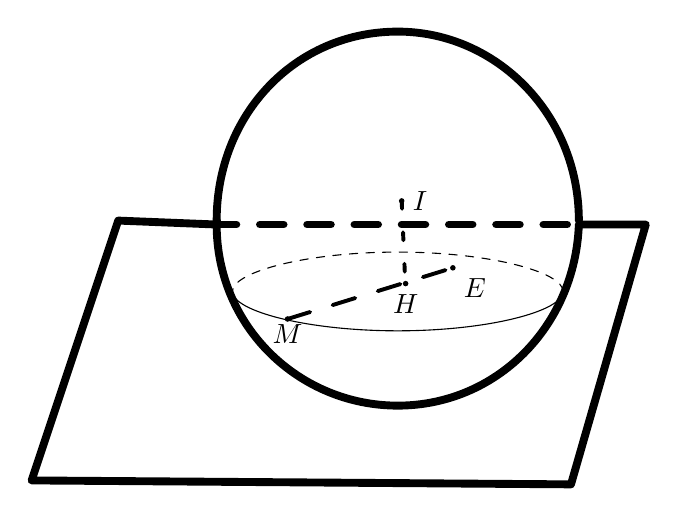
\begin{tikzpicture}[scale=.5, every node/.append style={scale=1}, line cap=round, line join=round, inner sep=0pt, outer sep=0pt]
				
				% Vỏ ngoài
				\draw[line width=1mm] 
				(17.5,12.1) .. controls (17.4,9.5) and (15.4,7.5) .. (12.9,7.5)
				.. controls (10.4,7.5) and (8.3,9.5) .. (8.3,12.1) --
				(5.8,12.2) -- (3.6,5.6) -- (17.3,5.5) -- (19.2,12.1) -- cycle;
				
				% Miệng trên
				\draw[line width=1mm] 
				(17.5,12.2) .. controls (17.5,14.9) and (15.4,17.0) .. (12.9,17.0)
				.. controls (10.3,17.0) and (8.3,14.9) .. (8.3,12.2);
				
				% Đường nét đứt phần miệng
				\draw[line width=1mm, dash pattern=on 3mm off 3mm] 
				(8.3,12.2) -- (8.3,12.1) -- (17.5,12.1) -- (17.5,12.2);
				
				% Vành trong trên
				\draw[dashed] 
				(17.1,10.4) .. controls (17.1,10.9) and (15.2,11.4) .. (12.9,11.4)
				.. controls (10.6,11.4) and (8.7,10.9) .. (8.7,10.4);
				
				% Vành trong dưới
				\draw 
				(8.7,10.4) .. controls (8.7,9.9) and (10.6,9.4) .. (12.9,9.4)
				.. controls (15.2,9.4) and (17.1,9.9) .. (17.1,10.4);
				
				% Đường nét đứt thẳng đứng
				\draw[line width=.5mm, dash pattern=on 1mm off 3mm] 
				(13.0,12.7) -- (13.1,10.4);
				\fill (10.1,9.7)circle(2pt) node[below=2pt]{$M$};
				\fill (13.1,10.6)circle(2pt) node[below=4pt]{$H$};
				\fill (14.3,11.0)circle(2pt) node[below right=4pt]{$E$};
				\fill (13.0,12.7)circle(2pt) node[right=4pt]{$I$};
				% Đường nét đứt xiên
				\draw[line width=.5mm, dash pattern=on 3mm off 3mm] 
				(10.1,9.7) -- (14.3,11.0);
				
			\end{tikzpicture}
		\end{center}
		Gọi $M(x;y;z)$.
		\begin{itemize}
			\item Tập hợp điểm $M$ thỏa mãn $MA = \sqrt{2} MB$ nên
			\begin{eqnarray*}
				&& \sqrt{(x - 1)^2 + (y - 1)^2 + (z - 2)^2} = \sqrt{2} \cdot \sqrt{(x + 1)^2 + (y - 2)^2 + (z - 1)^2} \\
				&\Leftrightarrow& (x - 1)^2 + (y - 1)^2 + (z - 2)^2 = 2\left[(x + 1)^2 + (y - 2)^2 + (z - 1)^2\right] \\
				&\Leftrightarrow& x^2 + y^2 + z^2 + 6x - 6y + 6 = 0.
			\end{eqnarray*}
			Phương trình mặt cầu tâm $I(-3; 3; 0)$, bán kính $R = 2\sqrt{3}$.	
			\item Gọi $H$ là hình chiếu vuông góc của $I$ lên $(P)$. \\
			Phương trình đường thẳng $d$ đi qua $I$ và vuông góc với $(P)$ là $\heva{&x=-3+t\\&y=3+t,\, t\in\mathbb{R}\\&z=t.}$\\
			Xét phương trình $(-3+t)+(3+t)+t-1=0\Leftrightarrow t=\dfrac{1}{3}$.\\
			Vậy $H\left(\dfrac{-8}{3};\dfrac{10}{3};\dfrac{1}{3}\right)$.
			\item Giao của mặt cầu với mặt phẳng $(P)$ với ($r$ là bán kính).
			\begin{eqnarray*}
				&& \mathrm{d}(I,(P)) = \dfrac{|-3 + 3 + 0 - 1|}{\sqrt{1^2 + 1^2 + 1^2}} = \dfrac{\sqrt{3}}{3} \\
				&& r = \sqrt{R^2 - d^2} = \dfrac{\sqrt{105}}{3}.
			\end{eqnarray*}
			\item Giá trị lớn nhất của $EM$. Dễ thấy điểm $E\in (P)$ và 
			\begin{eqnarray*}
				&& EH = \dfrac{\sqrt{6}}{3} \\
				&& EM_{\text{max}} = HE + r =\dfrac{\sqrt{6}}{3}+\dfrac{\sqrt{105}}{3}\approx 4{,}2.
			\end{eqnarray*}
		\end{itemize}
		Vậy giá trị lớn nhất của $EM$ là $4{,}2$.
	}
\end{ex}
%Câu 10
\begin{ex}[Trích đề thi HK2-THPT-Hướng Hóa-Quảng Trị-HKII-Năm học 2024-2025]%[2H5V3-4]%[Dự án đề cương 3 khối NH24-25 Đợt2-Nguyễn Tiến Liên]
	Các thiên thạch có đường kính lớn hơn $40$ m và có thể lại gần Trái Đất ở khoảng cách nhỏ hơn $7\, 500\, 000$ km được coi là những vật thể có khả năng va chạm gây nguy hiểm cho Trái Đất. Để theo dõi những thiên thạch này, người ta đã thiết lập các trạm quan sát các vật thể bay gần Trái Đất. Để theo dõi những thiên thạch này, người ta đã thiết lập các trạm quan sát các vật thể bay gần Trái Đất. Giả sử có một hệ thống quan sát có khả năng theo dõi các vật thể ở độ cao không vượt quá $6\,630$ km. Chọn hệ trục tọa độ $Oxyz$ trong không gian có gốc $O$ tại tâm Trái Đất và đơn vị trên mỗi trục tọa độ là $1\,000$ km. Một thiên thạch (coi như một hạt) chuyển động với tốc độ không đổi theo một đường thẳng từ điểm $M(-12;29;10)$ theo phương song song với giá của vectơ $\overrightarrow{u}=(-12;17;5)$. Vị trí cuối cùng mà thiên thạch di chuyển trong phạm vi theo dõi của hệ thống quan sát là điểm nào dưới đây?
	\begin{center}
		\begin{tikzpicture}[line join=round, line cap=round,>=stealth,scale=0.75]
			\path
			(0,0) coordinate (O)
			(-4,4) coordinate (M) node [above] {$M$}
			(1,3) coordinate (N)
			(6,2) coordinate (P)
			;
			\draw[name path=c] (O) circle (4)
			;
			\draw [fill=gray!50] (O) circle (2)
			;
			\draw[<->] (O)--(2,0) node [pos=.5, above] {$6\,370$ km};
			\draw [<->] (2,0)--(4,0) node [pos=.5, above] {$6\,630$ km};
			\draw [name path=a, thick, blue] (M)--(N);
			\draw [name path=b, thick, blue] (N)--(P);
			\path[name intersections={of=c and a}] (intersection-1) coordinate (A) node [below right] {$A$};
			\path[name intersections={of=c and b}] (intersection-1) coordinate (B) node [below left] {$B$};	
			\foreach \i in {A,B,M}\draw[fill=black] (\i)circle (1pt);
		\end{tikzpicture}
	\end{center}
	\choice
	{$B(12;0;-5)$}
	{$B(12;5;0)$}
	{\True$B(12;-5;0)$}
	{$B(0;12;5)$}
	\loigiai{Phương trình đường thẳng $AB\colon \heva{&x=-12-12t\\& y=29+17t\\&z=10+5t.}$\\
		Phương trình mặt cầu tâm $O(0;0;0)$, bán kính $R=\dfrac{6\ 370+6\ 630}{1\ 000}=13$ có dạng:
		\begin{center}
			$x^2+y^2+z^2=13^2$ hay $x^2+y^2+z^2=169$.
		\end{center}
		Tọa độ giao điểm của đường thẳng $AB$ và mặt cầu thỏa mãn
		\begin{center}
			$(-12-12t)^2+(29+17t)^2+(10+5t)^2=169\Leftrightarrow 458t^2+1\ 374t+916=0\Leftrightarrow\hoac{&t=-1\\&t=-2.}$
		\end{center}
		Suy ra tọa độ giao điểm của đường thẳng $AB$ và mặt cầu là $(0;12;5)$, $(12;-5;0)$.\\
		Do $x_B>x_A$ (vị trí cuối cùng mà thiên thạch đi qua) nên $B(12;-5;0)$.
	}
\end{ex}
%Câu 11
\begin{ex}[Trích đề thi HKII-THPT Chế Lan Viên - Quảng Trị-Năm học 2024-2025]%[2H5V3-4]%[Dự án đề cương 3 khối NH24-25 Đợt2-Nguyễn Tiến Liên]
	Trong không gian $Oxyz$, đài kiểm soát không lưu sân bay có tọa độ $O(0; 0; 0)$, mỗi đơn vị trên trục ứng với $1$ km. Máy bay bay trong phạm vi cách đài kiểm soát $417$ km sẽ hiển thị trên màn hình ra đa. Một máy bay đang ở vị trí $A(-688;-185;8)$, chuyển động theo đường thẳng $d$ có vectơ chỉ phương là $\overrightarrow{u}=(91; 75; 0)$ và hướng về đài kiểm soát không lưu. 
	\begin{center}
		\begin{tikzpicture}[scale=0.6, font=\footnotesize, line join=round, line cap=round, >=stealth] 
			\def\r{3}
			\def \x{3}  %bán kính trục lớn elip
			\def \y{1.2} 
			\coordinate (o1) at (-\r,0);
			\coordinate (o2) at (\r,0);
			\coordinate (O) at (0,0);
			% ve mp
			\coordinate (P) at (-5,2);
			\coordinate (Q) at ($(P)+(240:6)$);
			\coordinate (R) at ($(Q)+(12,0)$);
			\coordinate (S) at ($(R)+(60:6)$);
			\fill[cyan!20] (P)--(Q)--(R)--(S)--cycle;
			\draw (O) circle(\r); 
			\path[fill=orange!20] (O) circle(\r); 
			\fill[orange!80] (o2) arc (0:-180:\x cm and \y cm) arc (180:360:\x cm and \x cm);
			\draw[dashed] (o2) arc (0:180:\x cm and \y cm);
			\draw (o2) arc (0:-180:\x cm and \y cm);
			% truc oz
			\coordinate (Oz) at (0,4.5);
			\coordinate (Oz') at (0,2.5);
			\coordinate (Oz'') at (0,-3.5);
			\draw[dashed] (Oz'')--(Oz');
			\draw[->] (Oz')--(Oz);
			% tru  ox
			\def\t{240}
			\coordinate (Ox) at ({\x*cos(\t)},{\y*sin(\t)});
			\coordinate (Ox') at ($(O)!2!(Ox)$);
			\coordinate (Ox'') at ($(Ox)!2.2!(O)$);
			\draw[dashed] (O)--(Ox);
			\draw[->] (Ox)--(Ox');
			\draw[dashed] (O)--(Ox'');
			% truc oy
			\coordinate (O4) at (\r,0);
			\coordinate (O5) at (1.5*\r,0);
			\coordinate (O2) at (-\r,0);
			\coordinate (O1) at (-1.5*\r,0);
			\draw (O1)--(O2);
			\draw[dashed] (O2)--(O4);
			\draw[->] (O4)--(O5);
			% duong d
			\coordinate (A) at (-4.52,1.7);
			\coordinate (A3) at (4.5,0.3);
			\coordinate (A1) at ($(A)!0.25!(A3)$);
			\coordinate (A2) at ($(A)!0.82!(A3)$);
			\draw (A)--(A1);
			\draw[dashed] (A1)--(A2);
			\draw (A2)--(A3);
			\foreach \x in {O}{
				\fill (\x) circle(1pt);
			}
			\path 
			node at (O) [above left]{$O$}
			node at (A) [above] {$A$}
			node at (A1) [above right]{$B$}
			node at (A2) [above right]{$C$}
			node at (A3) [above]{$d$}
			node at (Oz) [left]{$z$}
			node at (O5) [below]{$y$}
			node at (Ox')[below]{$x$}
			;
		\end{tikzpicture}
	\end{center}
	Gọi $H(a;b;c)$ là vị trí mà máy bay gần đài kiểm soát không lưu nhất. Tính $S=a-b+c$.
	\loigiai{
		Đường thẳng $d$ đi qua $A(-688;-185;8)$, có véc-tơ chỉ phương là $\overrightarrow{u}=(91;75;0)$ nên có phương trình tham số là $$\heva{& x=-688 +91t \\&y=-185+75t\\&z=8.} \quad t\in \mathbb{R}$$\\
		Gọi $(P)$ là mặt phẳng đi qua $O$ và vuông góc với đường thẳng $d$. \\
		Ta có $(P)\perp d$ nên nhận véc-tơ chỉ phương của $d$ là một véc-tơ pháp tuyến.\\
		Vậy $(P)$ đi qua $O(0;0;0)$ và có véc-tơ pháp tuyến $\overrightarrow{n}_{P}=\overrightarrow{u}_d=(91;75;0)$ nên có phương trình 
		$$91\cdot (x-0)+75\cdot (y-0)+0\cdot (z-0)=0 \Leftrightarrow 91x+75y=0.$$
		Gọi $H$ là hình chiếu vuông góc của $O$ lên đường thẳng $d$, ta có $H$ là giao của đường thẳng $d$ và mặt phẳng $(P)$.\\
		 Khi đó tọa độ của $H$ là nghiệm của hệ phương trình 
		\begin{eqnarray*}
			\heva{&x=-688 +91t\\&y=-185+75t\\&z=8\\& 91x+75y=0} 
			\Leftrightarrow
			\heva{&x=-688 +91t\\&y=-185+75t\\ &z=8\\& 91 \cdot(-688 +91t)+75 \cdot (-185+75t)=0}  
			\Leftrightarrow\heva{&t=\dfrac{11}{2}\\& x=-\dfrac{375}{2}\\&y=\dfrac{455}{2}\\&z=8.}
		\end{eqnarray*}
		Vậy tọa độ của vị trí mà máy bay bay gần đài kiểm soát không lưu nhất là $H\left(-\dfrac{375}{2};\dfrac{455}{2};8\right)$.\\
		Do đó $a=-\dfrac{375}{2}$, $b=\dfrac{455}{2}$, $c=8$.\\
		 Vậy $a-b+c=-407$.
	}
\end{ex} 
%Câu 12
\begin{ex}[Trích đề thi HKII-Thuận Thành 1-Bắc Ninh-Năm học 2024-2025]%[2H5V3-4]%[Dự án đề cương 3 khối NH24-25 Đợt2-Nguyễn Tiến Liên]
	Một quả bóng rổ được đặt ở một góc của căn phòng hình hộp chữ nhật, sao cho quả bóng chạm và tiếp xúc với hai bức tường và nền nhà của căn phòng đó thì có một điểm trên quả bóng có khoảng cách lần lượt đến hai bức tường và nền nhà là $17$ cm, $18$ cm, $21$ cm (tham khảo hình minh họa). Hỏi độ dài đường kính của quả bóng bằng bao nhiêu cm biết rằng quả bóng rổ tiêu chuẩn có đường kính từ $23$ cm đến $24{,}5$ cm? (Kết quả là tròn đến chữ số thập phân thứ nhất).
	\begin{center}
		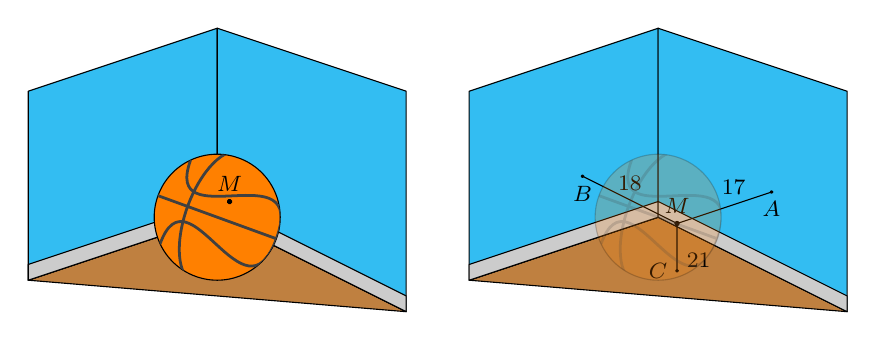
\begin{tikzpicture}[line join = round, line cap=round,>=stealth,font=\footnotesize,scale=0.8]			
			% === Hình bên trái ===
			\begin{scope}[shift={(-3.5,0)}]
				\draw[fill=brown] (-3,-1)--(0,0)--(3,-1.5)--cycle;
				\draw[fill=cyan!80] (-3,-1)--(0,0)--(0,3)--(-3,2)--cycle;
				\draw[fill=cyan!80] (3,-1.5)--(0,0)--(0,3)--(3,2)--cycle;
				\draw[fill=white!80!black] (0,0)--(0,0.25)--(-3,-0.75)--(-3,-1)--cycle;
				\draw[fill=white!80!black] (0,0)--(0,0.25)--(3,-1.25)--(3,-1.5)--cycle;
				\begin{scope}[rotate=70]
					\clip[preaction={draw=black,fill=orange}] (0,0) circle(1cm);	
					\fill (0.3,-0.1) circle(1.2pt)node[above]{$M$};
					\draw[black!75,line width=1pt] 
					(90:1) -- (270:1)
					(180:11/10) arc (180:0:11/10 and 1/2)
					(270:1) .. controls ++(180:3/2) and ++(0:4/3) ..(135:1)
					(270:1) .. controls ++(0:3/2) and ++(180:4/3) ..(45:1);
				\end{scope}
			\end{scope}
			% === Hình bên phải ===
			\begin{scope}[shift={(3.5,0)}]
				\draw[fill=brown] (-3,-1)--(0,0)--(3,-1.5)--cycle;
				\draw[fill=cyan!80] (-3,-1)--(0,0)--(0,3)--(-3,2)--cycle;
				\draw[fill=cyan!80] (3,-1.5)--(0,0)--(0,3)--(3,2)--cycle;
				\draw[fill=white!80!black] (0,0)--(0,0.25)--(-3,-0.75)--(-3,-1)--cycle;
				\draw[fill=white!80!black] (0,0)--(0,0.25)--(3,-1.25)--(3,-1.5)--cycle;
				\fill (0.3,-0.1) circle(1.2pt)node[above]{$M$};		
				\draw[shift={(0.3,-0.1)},scale=0.5] (0,0)--(0,-1.5) circle(1.2pt) node[left]{$C$} node[pos=0.78,right]{$21$}; 		
				\draw[shift={(0.3,-0.1)},scale=0.5,yshift=1cm,xshift=3cm] (-3,-1)--(0,0) circle(1.2pt) node[below]{$A$}node[pos=0.7,above,pos=0.6]{$17$}; 		
				\draw[shift={(0.3,-0.1)},scale=0.5,xshift=-3cm,yshift=1.5cm] (0,0)circle(1.2pt) node[below]{$B$}--(3,-1.5)node[pos=0.5,above]{$18$};	
				\begin{scope}[rotate=70,opacity=0.2]
					\clip[preaction={draw=black,fill=orange}] (0,0) circle(1cm);		
					\draw[black!75,line width=1pt] 
					(90:1) -- (270:1)
					(180:11/10) arc (180:0:11/10 and 1/2)
					(270:1) .. controls ++(180:3/2) and ++(0:4/3) ..(135:1)
					(270:1) .. controls ++(0:3/2) and ++(180:4/3) ..(45:1);
				\end{scope}
			\end{scope}
		\end{tikzpicture}		
	\end{center}
	\loigiai{
		Gọi tâm của quả bóng là $I$. Do quả bóng tiếp xúc với ba mặt của căn phòng (hai tường và sàn nhà), nên tâm $I$ cách đều ba mặt đó. Đặt hệ trục tọa độ $Oxyz$ sao cho:
		\begin{itemize}
			\item mặt phẳng $x = 0$ là một bức tường,
			\item mặt phẳng $y = 0$ là bức tường còn lại,
			\item mặt phẳng $z = 0$ là mặt sàn,
		\end{itemize}
		thì tâm $I$ của quả bóng có tọa độ $I(R; R; R)$, với $R$ là bán kính quả bóng.\\	
		Gọi điểm $M$ là điểm trên mặt cầu có khoảng cách đến ba mặt là
		$$x_M = 17,\quad y_M = 18,\quad z_M = 21 \Rightarrow M(17; 18; 21).$$
		Vì $M$ nằm trên mặt cầu tâm $I$ và bán kính $R$ nên
		$$IM = R = \sqrt{(17 - R)^2 + (18 - R)^2 + (21 - R)^2}.$$
		Suy ra
		\allowdisplaybreaks
		\begin{eqnarray*}
			&&R^2 = (17 - R)^2 + (18 - R)^2 + (21 - R)^2
			\\
			&\Leftrightarrow&2R^2 - 112R + 1054 = 0 
			\\
			&\Leftrightarrow& R^2 - 56R + 527 = 0
			\\
			&\Rightarrow&R = \dfrac{56 \pm \sqrt{1028}}{2}
			\\
			&\Rightarrow&R  \approx \dfrac{56 \pm 32{,}06}{2}.
		\end{eqnarray*}
		Lấy nghiệm phù hợp $R \approx \dfrac{56 - 32{,}06}{2} \approx 11{,}97$.\\
		Vậy đường kính của quả bóng là $2R \approx 24$ cm.
	}
\end{ex}
